% =====================================================================
% Supporting Information, ACS Omega resubmission (ao-2026-09173w) -- REBUILT AROUND THE N3 BENCHMARK, draft 2026-11-17
%
% EVERY NUMBER in this file enters through generated/si_*.tex, written by scripts/n3_si_tables.py from the named
% evidence records: results/n3/n3_results.json (committed f1c713a, before interpretation), n3_selection.json,
% table_r_{testB,devtest}.json, gateF.json, gateC.json, omc25_outside_elements_{testB,devtest}.json and, for the
% run-health counts that no results file holds, tasks/n3_step4_record_2026-10-11.md (each such macro in
% generated/si_numbers.tex cites the record by file:line). Regenerate with `python scripts/n3_si_tables.py`;
% `--check` exits 0 when the generated files are current. Each table below carries a `% src:` comment, and each
% generated file repeats its source keys. Method parameters (seeds, S = 16, stol values, tolerances, the
% "3-model ensemble, 48 draws" label) are typed and labelled as parameters.
% CLAIM RULES: tasks/n3_protocol.md Section 2.4 -- no significance language for secondary matchers, draw@1, any@k,
% ensembles, continuous endpoints, strata, DEV-TEST, MCF-A, ablations or diagnostics (contract assertion 5).
% Section S1 is sections/si_n3.tex (not edited here). The pre-N3 SI is archived in
% archive/si-archive-2026-11-17-pre-N3.tex and archive/si-archive-2026-11-17-pre-N3-b.tex.
%
% achemso's acsodf configuration declares \acs@type@list{article} only (achemso-acsodf.cfg:25), so
% manuscript=suppinfo silently falls back to article; we load article and set the S-prefixed counters ourselves.
% =====================================================================
\documentclass[journal=acsodf,manuscript=article]{achemso}

\usepackage{amsmath,amssymb}
\usepackage{graphicx}
\usepackage{booktabs}
\usepackage{xcolor}
\usepackage{rotating}
\usepackage{array}
\usepackage{longtable}
\usepackage{pgfplots}
\pgfplotsset{compat=1.18}
\graphicspath{{figures/}{../../figures/}}

% --- achemso `suppinfo` behaviour under the acsodf configuration ---------
\AbstractOff
\renewcommand{\thesection}{S\arabic{section}}
\renewcommand{\thesubsection}{S\arabic{section}.\arabic{subsection}}
\renewcommand{\thetable}{S\arabic{table}}
\renewcommand{\thefigure}{S\arabic{figure}}
\renewcommand{\theequation}{S\arabic{equation}}
% ---------------------------------------------------------------------------

% GENERATED by scripts/n3_si_tables.py from the named N3 evidence records -- do not edit
\newcommand{\svN}{1{,}000}% src: results/n3/n3_results.json sets.testB.report.n
\newcommand{\svNDev}{200}% src: results/n3/n3_results.json sets.devtest.report.n
\newcommand{\svOursSel}{LJ}% src: results/n3/n3_selection.json frozen.OURS.selector (= OURS-N2)
\newcommand{\svOursS}{16}% src: results/n3/n3_selection.json frozen.OURS.S (= OURS-N2)
\newcommand{\svOursEuler}{40}% src: results/n3/n3_selection.json frozen.OURS.euler_steps (= OURS-N2)
\newcommand{\svOursEpochs}{8}% src: frozen OURS checkpoints results/vast_g2/eval_s0.pt (s0-s2; SHA-256 checked) hist (epoch, val, sec) and best; results/g2_learned_s{s}.resume.pt, results/vast_g2/g2_learned_s{s}.resume.pt (epochs run locally / in all); CPU (scripts/g2_learned_flow.py has no device option)
\newcommand{\svOursBestEpochs}{1, 8 and 4}% src: frozen OURS checkpoints results/vast_g2/eval_s0.pt (s0-s2; SHA-256 checked) hist (epoch, val, sec) and best; results/g2_learned_s{s}.resume.pt, results/vast_g2/g2_learned_s{s}.resume.pt (epochs run locally / in all); CPU (scripts/g2_learned_flow.py has no device option) (argmin val, one-based, seeds 0/1/2)
\newcommand{\svOursRanEpochs}{9}% src: frozen OURS checkpoints results/vast_g2/eval_s0.pt (s0-s2; SHA-256 checked) hist (epoch, val, sec) and best; results/g2_learned_s{s}.resume.pt, results/vast_g2/g2_learned_s{s}.resume.pt (epochs run locally / in all); CPU (scripts/g2_learned_flow.py has no device option)
\newcommand{\svOursLocalEpochs}{3}% src: frozen OURS checkpoints results/vast_g2/eval_s0.pt (s0-s2; SHA-256 checked) hist (epoch, val, sec) and best; results/g2_learned_s{s}.resume.pt, results/vast_g2/g2_learned_s{s}.resume.pt (epochs run locally / in all); CPU (scripts/g2_learned_flow.py has no device option)
\newcommand{\svOursNTwoEpochs}{30}% src: results/vast_n12/n2_s{0,1,2}.json (args.epochs, args.procs, hist sec); frozen OURS-N2 checkpoints matched tensor-wise to results/vast_n12/n2_s<s>.pt best_state or .resume.pt model; CPU (gloo, scripts/g2_train_v2.py)
\newcommand{\svOursNTwoChosen}{30, 30 and 25}% src: results/vast_n12/n2_s{0,1,2}.json (args.epochs, args.procs, hist sec); frozen OURS-N2 checkpoints matched tensor-wise to results/vast_n12/n2_s<s>.pt best_state or .resume.pt model; CPU (gloo, scripts/g2_train_v2.py) (one-based, seeds 0/1/2)
\newcommand{\svTrainOursSeed}{2.87--2.90}% src: frozen OURS checkpoints results/vast_g2/eval_s0.pt (s0-s2; SHA-256 checked) hist (epoch, val, sec) and best; results/g2_learned_s{s}.resume.pt, results/vast_g2/g2_learned_s{s}.resume.pt (epochs run locally / in all); CPU (scripts/g2_learned_flow.py has no device option) (h per seed)
\newcommand{\svTrainNTwoSeed}{1.63--1.64}% src: results/vast_n12/n2_s{0,1,2}.json (args.epochs, args.procs, hist sec); frozen OURS-N2 checkpoints matched tensor-wise to results/vast_n12/n2_s<s>.pt best_state or .resume.pt model; CPU (gloo, scripts/g2_train_v2.py) (h per seed)
\newcommand{\svTrainNTwoProcs}{16}% src: results/vast_n12/n2_s{0,1,2}.json (args.epochs, args.procs, hist sec); frozen OURS-N2 checkpoints matched tensor-wise to results/vast_n12/n2_s<s>.pt best_state or .resume.pt model; CPU (gloo, scripts/g2_train_v2.py)
\newcommand{\svTrainMcfRSeed}{1.34--1.36}% src: n3_mcf/runs/n3_mcfR_s{0,1,2}_train.json hours (training-process wall-clock) and .log (one device) (h per seed)
\newcommand{\svTrainMcfASeed}{1.82--1.83}% src: n3_mcf/runs/n3_mcfA_s{0,1,2}_train.json hours (training-process wall-clock) and .log (one device) (h per seed)
\newcommand{\svTrainIvPSeed}{0.13}% src: results/n3/private/old/runs/<run>/hist.jsonl (sum of per-epoch sec) and meta.json (device cuda); runs of record from results/n3/n3_selection.json frozen.iv-P.checkpoints (h per seed)
\newcommand{\svTrainIvPScreen}{0.25}% src: results/n3/private/old/runs/<run>/hist.jsonl (sum of per-epoch sec) and meta.json (device cuda); runs of record from results/n3/n3_selection.json frozen.iv-P.checkpoints (learning-rate screening runs lr1e-3_s0, lr3e-4_s0)
\newcommand{\svGtwoContext}{G2 DEV-TEST: basin\_best 10.1/8.5/7.0\% vs Haar 6.5\%, p = 0.19/0.54/1.0; basin\_any 22.6/19.6/17.6\% vs 11.1\%}% src: results/n3/n3_results.json sets.testB.report.steric_basin.g2_devtest_context (its trailing cross-reference to the protocol dropped)
\newcommand{\svDecTot}{+8.33}% src: results/n3/n3_results.json sets.testB.report.table1.MCF-R+G.delta_ours_minus_arm.delta_pp
\newcommand{\svDecTotCI}{[7.30, 9.40]}% src: results/n3/n3_results.json sets.testB.report.table1.MCF-R+G.delta_ours_minus_arm.bca_pp
\newcommand{\svDecExp}{+0.83}% src: results/n3/n3_results.json sets.testB.report.wording.ii_S_decomposition.'ii-S - MCF-R+G'.delta_pp
\newcommand{\svDecExpCI}{[0.53, 1.20]}% src: results/n3/n3_results.json sets.testB.report.wording.ii_S_decomposition.'ii-S - MCF-R+G'.bca_pp
\newcommand{\svDecLearn}{+7.50}% src: results/n3/n3_results.json sets.testB.report.wording.ii_S_decomposition.'OURS - ii-S'.delta_pp
\newcommand{\svDecLearnCI}{[6.47, 8.65]}% src: results/n3/n3_results.json sets.testB.report.wording.ii_S_decomposition.'OURS - ii-S'.bca_pp
\newcommand{\svDecompSum}{+8.33}% src: results/n3/n3_results.json sets.testB.report.wording.ii_S_decomposition: (ii-S - MCF-R+G) + (OURS - ii-S), delta_pp
\newcommand{\svDecompLearner}{adds}% src: results/n3/n3_results.json sets.testB.report.wording.ii_S_decomposition.learner
\newcommand{\svZmcfMin}{+8.18}% src: results/n3/n3_results.json sets.testB.report.wording.zmcf_ge3_min_delta_pp
\newcommand{\svBasinUnconvN}{15}% src: results/n3/n3_results.json sets.testB.report.h2_basin_reference.ref_unconverged_refcodes (count)
\newcommand{\svBasinUnconv}{OPEDAP, TIKXIW, OHEDEK, OBEZAZ, DETNEW, KEBCIH, VURYEQ, XICRIO, MEKJAN, GUNLIO, FURNEP, PEWQIT, BEYZAG, IXESEL01, TIFGEV}% src: results/n3/n3_results.json sets.testB.report.h2_basin_reference.ref_unconverged_refcodes
\newcommand{\svBasinInvalid}{none}% src: results/n3/n3_results.json sets.testB.report.h2_basin_reference.ref_invalid_refcodes
\newcommand{\svOmcN}{818}% src: results/n3/n3_results.json sets.testB.report.h2_omc25_nonoverlap.n
\newcommand{\svDiagBNote}{c\_i does NOT bound LJ-picked@1}% src: results/n3/n3_results.json sets.testB.mcf_diagnostics.b.note
\newcommand{\svDiagBGrid}{5}% src: results/n3/n3_results.json sets.testB.mcf_diagnostics.b.grid_deg
\newcommand{\svDiagBWalk}{1}% src: results/n3/n3_results.json sets.testB.mcf_diagnostics.b.walk_deg
\newcommand{\svDiagCZoneN}{5}% src: results/n3/n3_results.json sets.testB.mcf_diagnostics.c.'z_MCF = 1'.n
\newcommand{\svDiagDConsistent}{yes}% src: results/n3/n3_results.json sets.testB.mcf_diagnostics.d_consistent_all
\newcommand{\svIiisArmFail}{285}% src: results/n3/n3_results.json sets.testB.report.table1.iii-s.arm_fail_draws
\newcommand{\svOmcOutside}{16}% src: results/n3/omc25_outside_elements_testB.json n_outside
\newcommand{\svOmcElements}{B, Br, C, Cl, F, H, I, N, O, P, S, Si}% src: results/n3/omc25_outside_elements_testB.json omc25_element_set
\newcommand{\svIiisFFSec}{85.44}% src: results/n3/private/classical/iii-s_testB.jsonl stats.sec (FF* call time only, median over crystals)
\newcommand{\svXHSetCH}{16{,}493}% src: results/n3/private/draws/<bundle>.pt meta.xh summed over crystals (= meta.xh_total where present), identical in every FF* run on TEST-B: basin-ours_n2_s0_testB.pt, basin-ours_n2_s1_testB.pt, basin-ours_n2_s2_testB.pt, fftruth_s-1_testB.pt, i-E-ours_s0_testB.pt, i-E-ours_s1_testB.pt, i-E-ours_s2_testB.pt, iii-s_s-1_testB.pt
\newcommand{\svXHSetNH}{422}% src: results/n3/private/draws/<bundle>.pt meta.xh summed over crystals (= meta.xh_total where present), identical in every FF* run on TEST-B: basin-ours_n2_s0_testB.pt, basin-ours_n2_s1_testB.pt, basin-ours_n2_s2_testB.pt, fftruth_s-1_testB.pt, i-E-ours_s0_testB.pt, i-E-ours_s1_testB.pt, i-E-ours_s2_testB.pt, iii-s_s-1_testB.pt
\newcommand{\svXHSetOH}{298}% src: results/n3/private/draws/<bundle>.pt meta.xh summed over crystals (= meta.xh_total where present), identical in every FF* run on TEST-B: basin-ours_n2_s0_testB.pt, basin-ours_n2_s1_testB.pt, basin-ours_n2_s2_testB.pt, fftruth_s-1_testB.pt, i-E-ours_s0_testB.pt, i-E-ours_s1_testB.pt, i-E-ours_s2_testB.pt, iii-s_s-1_testB.pt
\newcommand{\svXHSetShort}{213}% src: results/n3/private/draws/<bundle>.pt meta.xh summed over crystals (= meta.xh_total where present), identical in every FF* run on TEST-B: basin-ours_n2_s0_testB.pt, basin-ours_n2_s1_testB.pt, basin-ours_n2_s2_testB.pt, fftruth_s-1_testB.pt, i-E-ours_s0_testB.pt, i-E-ours_s1_testB.pt, i-E-ours_s2_testB.pt, iii-s_s-1_testB.pt
\newcommand{\svSpacingMcfA}{13, 2 and 7}% src: results/n3/private/draws/<bundle>.pt meta.lj_counts.spacing_inf (n3_mcf_run.py to_bundle: generated cell height < 2.5 A -> +inf), MCF-A seeds 0/1/2: mcfA_ep752_st10542_u3_f9_s0_testB.pt, mcfA_last_u3_f9_s1_testB.pt, mcfA_ep1195_st16744_u3_f9_s2_testB.pt
\newcommand{\svSpacingMcfAFloor}{11, 17 and 12}% src: results/n3/private/draws/<bundle>.pt meta.lj_counts.spacing_inf (n3_mcf_run.py to_bundle: generated cell height < 2.5 A -> +inf), MCF-A-floor seeds 0/1/2: mcfAfloor_s0_testB.pt, mcfAfloor_s1_testB.pt, mcfAfloor_s2_testB.pt
\newcommand{\svSpacingDraws}{16{,}000}% src: results/n3/n3_results.json sets.testB.report.n x 16 draws per seed (all valid)
\newcommand{\svGtwoContextDev}{G2 DEV-TEST: basin\_best 10.1/8.5/7.0\% vs Haar 6.5\%, p = 0.19/0.54/1.0; basin\_any 22.6/19.6/17.6\% vs 11.1\%}% src: results/n3/n3_results.json sets.devtest.report.steric_basin.g2_devtest_context (its trailing cross-reference to the protocol dropped)
\newcommand{\svBasinUnconvNDev}{1}% src: results/n3/n3_results.json sets.devtest.report.h2_basin_reference.ref_unconverged_refcodes (count)
\newcommand{\svBasinUnconvDev}{UYEZEE}% src: results/n3/n3_results.json sets.devtest.report.h2_basin_reference.ref_unconverged_refcodes
\newcommand{\svBasinInvalidDev}{none}% src: results/n3/n3_results.json sets.devtest.report.h2_basin_reference.ref_invalid_refcodes
\newcommand{\svOmcNDev}{164}% src: results/n3/n3_results.json sets.devtest.report.h2_omc25_nonoverlap.n
\newcommand{\svDiagBNoteDev}{c\_i does NOT bound LJ-picked@1}% src: results/n3/n3_results.json sets.devtest.mcf_diagnostics.b.note
\newcommand{\svDiagBGridDev}{5}% src: results/n3/n3_results.json sets.devtest.mcf_diagnostics.b.grid_deg
\newcommand{\svDiagBWalkDev}{1}% src: results/n3/n3_results.json sets.devtest.mcf_diagnostics.b.walk_deg
\newcommand{\svDiagCZoneNDev}{0}% src: results/n3/n3_results.json sets.devtest.mcf_diagnostics.c.'z_MCF = 1'.n
\newcommand{\svDiagDConsistentDev}{yes}% src: results/n3/n3_results.json sets.devtest.mcf_diagnostics.d_consistent_all
\newcommand{\svIiisArmFailDev}{107}% src: results/n3/n3_results.json sets.devtest.report.table1.iii-s.arm_fail_draws
\newcommand{\svOmcOutsideDev}{1}% src: results/n3/omc25_outside_elements_devtest.json n_outside
\newcommand{\svIiisFFSecDev}{81.15}% src: results/n3/private/classical/iii-s_devtest.jsonl stats.sec (FF* call time only, median over crystals)
\newcommand{\svXHSetCHDev}{3{,}166}% src: results/n3/private/draws/<bundle>.pt meta.xh summed over crystals (= meta.xh_total where present), identical in every FF* run on DEV-TEST: basin-ours_n2_s0_devtest.pt, basin-ours_n2_s1_devtest.pt, basin-ours_n2_s2_devtest.pt, fftruth_s-1_devtest.pt, i-E-ours_s0_devtest.pt, i-E-ours_s1_devtest.pt, i-E-ours_s2_devtest.pt, iii-s_s-1_devtest.pt
\newcommand{\svXHSetNHDev}{89}% src: results/n3/private/draws/<bundle>.pt meta.xh summed over crystals (= meta.xh_total where present), identical in every FF* run on DEV-TEST: basin-ours_n2_s0_devtest.pt, basin-ours_n2_s1_devtest.pt, basin-ours_n2_s2_devtest.pt, fftruth_s-1_devtest.pt, i-E-ours_s0_devtest.pt, i-E-ours_s1_devtest.pt, i-E-ours_s2_devtest.pt, iii-s_s-1_devtest.pt
\newcommand{\svXHSetOHDev}{52}% src: results/n3/private/draws/<bundle>.pt meta.xh summed over crystals (= meta.xh_total where present), identical in every FF* run on DEV-TEST: basin-ours_n2_s0_devtest.pt, basin-ours_n2_s1_devtest.pt, basin-ours_n2_s2_devtest.pt, fftruth_s-1_devtest.pt, i-E-ours_s0_devtest.pt, i-E-ours_s1_devtest.pt, i-E-ours_s2_devtest.pt, iii-s_s-1_devtest.pt
\newcommand{\svXHSetShortDev}{30}% src: results/n3/private/draws/<bundle>.pt meta.xh summed over crystals (= meta.xh_total where present), identical in every FF* run on DEV-TEST: basin-ours_n2_s0_devtest.pt, basin-ours_n2_s1_devtest.pt, basin-ours_n2_s2_devtest.pt, fftruth_s-1_devtest.pt, i-E-ours_s0_devtest.pt, i-E-ours_s1_devtest.pt, i-E-ours_s2_devtest.pt, iii-s_s-1_devtest.pt
\newcommand{\svSpacingMcfADev}{2, 1 and 1}% src: results/n3/private/draws/<bundle>.pt meta.lj_counts.spacing_inf (n3_mcf_run.py to_bundle: generated cell height < 2.5 A -> +inf), MCF-A seeds 0/1/2: mcfA_ep752_st10542_u3_f9_s0_devtest.pt, mcfA_last_u3_f9_s1_devtest.pt, mcfA_ep1195_st16744_u3_f9_s2_devtest.pt
\newcommand{\svSpacingMcfAFloorDev}{4, 3 and 2}% src: results/n3/private/draws/<bundle>.pt meta.lj_counts.spacing_inf (n3_mcf_run.py to_bundle: generated cell height < 2.5 A -> +inf), MCF-A-floor seeds 0/1/2: mcfAfloor_s0_devtest.pt, mcfAfloor_s1_devtest.pt, mcfAfloor_s2_devtest.pt
\newcommand{\svSpacingDrawsDev}{3{,}200}% src: results/n3/n3_results.json sets.devtest.report.n x 16 draws per seed (all valid)
\newcommand{\svOursSec}{16.76}% src: results/n3/n3_results.json sets.testB.report.table1.OURS.compute.sec_per_crystal_per_seed_median
\newcommand{\svOursLj}{16}% src: results/n3/n3_results.json sets.testB.report.table1.OURS.compute.lj_evals_per_crystal
\newcommand{\svTolQ}{$1.0\times10^{-6}$}% src: results/n3/n3_results.json mcf_diagnostic_a.per_checkpoint.mcfR_s0.tolerances.q (identical for all)
\newcommand{\svTolLat}{$1.0\times10^{-6}$}% src: results/n3/n3_results.json mcf_diagnostic_a.per_checkpoint.mcfR_s0.tolerances.lat (identical for all)
\newcommand{\svTolTr}{$1.0\times10^{-6}$}% src: results/n3/n3_results.json mcf_diagnostic_a.per_checkpoint.mcfR_s0.tolerances.tr (identical for all)
\newcommand{\svTolR}{$1.0\times10^{-5}$}% src: results/n3/n3_results.json mcf_diagnostic_a.per_checkpoint.mcfR_s0.tolerances.R (identical for all)
\newcommand{\svDiagAVerdict}{PASS}% src: results/n3/n3_results.json mcf_diagnostic_a.verdict
\newcommand{\svDiagAApproxN}{7}% src: results/n3/n3_results.json mcf_diagnostic_a.approximate_checkpoints (count)
\newcommand{\svDiagAApprox}{MCF-R s0, MCF-R s1, MCF-R s2, MCF-R+G s0, MCF-A s0, MCF-A s1, MCF-A s2}% src: results/n3/n3_results.json mcf_diagnostic_a.approximate_checkpoints
\newcommand{\svThreads}{32}% src: results/n3/n3_results.json mcf_diagnostic_a.per_checkpoint.*.torch_threads
\newcommand{\svForkSets}{VAL, DEV-TEST, TRAIN, VALSEL, TEST-B}% src: results/n3/gateF.json sets.<set>.p1_maps_patched
\newcommand{\svMcfBase}{3c493f8}% src: results/n3/gateF.json sets.testB.mcf_base
\newcommand{\svTRN}{649}% src: results/n3/table_r_testB.json wording.N_legacy_unrep
\newcommand{\svTRM}{604}% src: results/n3/table_r_testB.json wording.M_legacy_unrep_centro
\newcommand{\svTRNOracle}{658}% src: results/n3/table_r_testB.json wording.N_flag_or_oracle_miss
\newcommand{\svTRMOracle}{613}% src: results/n3/table_r_testB.json wording.M_flag_or_oracle_miss
\newcommand{\svTRMixed}{634}% src: results/n3/table_r_testB.json wording.n_mixed
\newcommand{\svTRP}{634}% src: results/n3/table_r_testB.json wording.P_mixed_not_matched_primary
\newcommand{\svTRQ}{323}% src: results/n3/table_r_testB.json wording.Q_mixed_matched_stol0.5
\newcommand{\svTRPSixteen}{634}% src: results/n3/table_r_testB.json wording.P_frozen16
\newcommand{\svTRQSixteen}{320}% src: results/n3/table_r_testB.json wording.Q_frozen16
\newcommand{\svTRUnres}{0}% src: results/n3/table_r_testB.json wording.mixed_c_unresolved
\newcommand{\svTROracleUnres}{0}% src: results/n3/table_r_testB.json wording.oracle_unresolved_flag_kept
\newcommand{\svTRText}{The legacy det+1 pipeline cannot represent 649/1000 test crystals (604 of the centrosymmetric ones). The released MolCrystalFlow CSP driver cannot produce 634/634 mixed-handedness cells under the default StructureMatcher; a homochiral approximant nevertheless matches 323/634 at stol 0.5.}% src: results/n3/table_r_testB.json wording.text
\newcommand{\svTRTextSixteen}{The legacy det+1 pipeline cannot represent 649/1000 test crystals (604 of the centrosymmetric ones). The released MolCrystalFlow CSP driver cannot produce 634/634 mixed-handedness cells under the default StructureMatcher; a homochiral approximant nevertheless matches 320/634 at stol 0.5.}% src: results/n3/table_r_testB.json wording.text_frozen16
\newcommand{\svTRImproperOk}{730}% src: results/n3/table_r_testB.json c_diagnostics.n_improper_ok
\newcommand{\svTRAutoImproved}{12}% src: results/n3/table_r_testB.json c_diagnostics.improved_by_automorphism_start_1e-6
\newcommand{\svTRChangedHalf}{3}% src: results/n3/table_r_testB.json c_diagnostics.outcome_changed_vs_frozen16.stol0.5
\newcommand{\svTRChangedPrimary}{0}% src: results/n3/table_r_testB.json c_diagnostics.outcome_changed_vs_frozen16.primary
\newcommand{\svTRMaxGain}{0.0797}% src: results/n3/table_r_testB.json c_diagnostics.max_rmsd_gain_A
\newcommand{\svTRRmsdMedMixed}{1.25}% src: results/n3/table_r_testB.json c_diagnostics.homochiral_rmsd.median_mixed
\newcommand{\svTRBad}{0}% src: results/n3/table_r_testB.json rows.*.{a,b,c,c_frozen16}.{timeout,deterministic,error,missing} + rows.*.d.oracle_* (sum)
\newcommand{\svTRByConstruction}{yes}% src: results/n3/table_r_testB.json a_by_construction
\newcommand{\svTRTimeout}{600}% src: results/n3/table_r_testB.json timing_s.timeout_per_job
\newcommand{\svTRNDev}{143}% src: results/n3/table_r_devtest.json wording.N_legacy_unrep
\newcommand{\svTRMDev}{131}% src: results/n3/table_r_devtest.json wording.M_legacy_unrep_centro
\newcommand{\svTRNOracleDev}{144}% src: results/n3/table_r_devtest.json wording.N_flag_or_oracle_miss
\newcommand{\svTRMOracleDev}{132}% src: results/n3/table_r_devtest.json wording.M_flag_or_oracle_miss
\newcommand{\svTRMixedDev}{137}% src: results/n3/table_r_devtest.json wording.n_mixed
\newcommand{\svTRPDev}{136}% src: results/n3/table_r_devtest.json wording.P_mixed_not_matched_primary
\newcommand{\svTRQDev}{83}% src: results/n3/table_r_devtest.json wording.Q_mixed_matched_stol0.5
\newcommand{\svTRPSixteenDev}{136}% src: results/n3/table_r_devtest.json wording.P_frozen16
\newcommand{\svTRQSixteenDev}{82}% src: results/n3/table_r_devtest.json wording.Q_frozen16
\newcommand{\svTRUnresDev}{0}% src: results/n3/table_r_devtest.json wording.mixed_c_unresolved
\newcommand{\svTROracleUnresDev}{0}% src: results/n3/table_r_devtest.json wording.oracle_unresolved_flag_kept
\newcommand{\svTRTextDev}{The legacy det+1 pipeline cannot represent 143/200 test crystals (131 of the centrosymmetric ones). The released MolCrystalFlow CSP driver cannot produce 136/137 mixed-handedness cells under the default StructureMatcher; a homochiral approximant nevertheless matches 83/137 at stol 0.5.}% src: results/n3/table_r_devtest.json wording.text
\newcommand{\svTRTextSixteenDev}{The legacy det+1 pipeline cannot represent 143/200 test crystals (131 of the centrosymmetric ones). The released MolCrystalFlow CSP driver cannot produce 136/137 mixed-handedness cells under the default StructureMatcher; a homochiral approximant nevertheless matches 82/137 at stol 0.5.}% src: results/n3/table_r_devtest.json wording.text_frozen16
\newcommand{\svTRImproperOkDev}{156}% src: results/n3/table_r_devtest.json c_diagnostics.n_improper_ok
\newcommand{\svTRAutoImprovedDev}{1}% src: results/n3/table_r_devtest.json c_diagnostics.improved_by_automorphism_start_1e-6
\newcommand{\svTRChangedHalfDev}{1}% src: results/n3/table_r_devtest.json c_diagnostics.outcome_changed_vs_frozen16.stol0.5
\newcommand{\svTRChangedPrimaryDev}{0}% src: results/n3/table_r_devtest.json c_diagnostics.outcome_changed_vs_frozen16.primary
\newcommand{\svTRMaxGainDev}{0.0555}% src: results/n3/table_r_devtest.json c_diagnostics.max_rmsd_gain_A
\newcommand{\svTRRmsdMedMixedDev}{1.15}% src: results/n3/table_r_devtest.json c_diagnostics.homochiral_rmsd.median_mixed
\newcommand{\svTRBadDev}{0}% src: results/n3/table_r_devtest.json rows.*.{a,b,c,c_frozen16}.{timeout,deterministic,error,missing} + rows.*.d.oracle_* (sum)
\newcommand{\svTRByConstructionDev}{no (computed)}% src: results/n3/table_r_devtest.json a_by_construction
\newcommand{\svTRTimeoutDev}{600}% src: results/n3/table_r_devtest.json timing_s.timeout_per_job
\newcommand{\svDevCifs}{3{,}500}% src: results/n3/table_r_testB.json corpus_context.dev.cifs
\newcommand{\svDevDetOne}{1{,}144}% src: results/n3/table_r_testB.json corpus_context.dev.kept_det1
\newcommand{\svDevOThree}{2{,}852}% src: results/n3/table_r_testB.json corpus_context.dev.kept_o3
\newcommand{\svDevEligible}{1{,}987}% src: results/n3/table_r_testB.json corpus_context.dev.eligible_g2_asym
\newcommand{\svDevNotEligible}{865}% src: results/n3/table_r_testB.json corpus_context.dev.o3_kept_not_eligible
\newcommand{\svPoolDetOne}{1{,}466}% src: results/n3/table_r_testB.json corpus_context.pool.kept_det1
\newcommand{\svValselN}{400}% src: results/n3/n3_selection.json valsel_cell_scores.<grid>.stage_a.table[*].n
\newcommand{\svIvPWindow}{30}% src: results/n3/n3_selection.json valsel_cell_scores.ivP_window.window
\newcommand{\svIvPLate}{no}% src: results/n3/n3_selection.json valsel_cell_scores.ivP_window.late_extension
\newcommand{\svFFRetryTotal}{1{,}208}% src: tasks/n3_step4_record_2026-10-11.md:871-872
\newcommand{\svFFRetryT}{640}% src: tasks/n3_step4_record_2026-10-11.md:871-872 (7S = iii-s/testB)
\newcommand{\svFFRetryD}{568}% src: tasks/n3_step4_record_2026-10-11.md:871-872 (7Sd = iii-s/devtest)
\newcommand{\svFFRetryBatch}{64}% src: tasks/n3_step4_record_2026-10-11.md:871-872
\newcommand{\svFFDet}{0}% src: tasks/n3_step4_record_2026-10-11.md:871-872
\newcommand{\svMcfCalls}{14}% src: tasks/n3_step4_record_2026-10-11.md:767-768
\newcommand{\svMcfNonfiniteDraws}{0}% src: tasks/n3_step4_record_2026-10-11.md:767-768
\newcommand{\svBranchClean}{13}% src: tasks/n3_step4_record_2026-10-11.md:769
\newcommand{\svBranchDraws}{1}% src: tasks/n3_step4_record_2026-10-11.md:769
\newcommand{\svBranchOf}{16{,}000}% src: tasks/n3_step4_record_2026-10-11.md:769
\newcommand{\svBranchCkpt}{ep1331}% src: tasks/n3_step4_record_2026-10-11.md:769
\newcommand{\svLJBundles}{24}% src: tasks/n3_step4_record_2026-10-11.md:771
\newcommand{\svLJDetFail}{0}% src: tasks/n3_step4_record_2026-10-11.md:771
\newcommand{\svLJNonfinite}{0}% src: tasks/n3_step4_record_2026-10-11.md:771
\newcommand{\svXHCH}{1{,}435}% src: tasks/n3_step4_record_2026-10-11.md:537-538
\newcommand{\svXHNH}{35}% src: tasks/n3_step4_record_2026-10-11.md:537-538
\newcommand{\svXHOH}{31}% src: tasks/n3_step4_record_2026-10-11.md:537-538
\newcommand{\svXHShort}{48}% src: tasks/n3_step4_record_2026-10-11.md:537-538
\newcommand{\svXHIeN}{2}% src: tasks/n3_step4_record_2026-10-11.md:644
\newcommand{\svXHIeCH}{34}% src: tasks/n3_step4_record_2026-10-11.md:644
\newcommand{\svAnchValOnly}{100.0}% src: results/n3/n3_results.json h2_form.anchoring_val_only
\newcommand{\svFairchem}{2.23.0}% src: results/n3/n3_results.json h2_form.fairchem_core
\newcommand{\svFFSettings}{batch, float32, cuda}% src: results/n3/n3_results.json h2_form.ffident
\newcommand{\svGcaAgree}{11{,}250/11{,}250}% src: results/n3/gateC.json C-a.labels.test.agreement
\newcommand{\svGcaAgreeVal}{11{,}070/11{,}070}% src: results/n3/gateC.json C-a.labels.val.agreement
\newcommand{\svGcbCpu}{36/36}% src: results/n3/gateC.json C-b.cpu.(bitwise_equal, tensors)
\newcommand{\svGcbRuns}{20}% src: results/n3/gateC.json C-b.cuda.runs
\newcommand{\svGcbStat}{3.02}% src: results/n3/gateC.json C-b.cuda.stat_patched
\newcommand{\svGcbMaxUn}{36.2}% src: results/n3/gateC.json C-b.cuda.stat_unpatched (max)
\newcommand{\svGcbBound}{0.05}% src: results/n3/gateC.json C-b.cuda.false_fail_bound
\newcommand{\svGcc}{16/16 lattices and 16/16 translations bitwise identical on 750 crystals}% src: results/n3/gateC.json C-c.(lattice_bitwise, trans_bitwise, S, n)
\newcommand{\svScoreEnv}{Python 3.12.15, PyTorch 2.11.0+cu128, pymatgen 2026.5.4, SciPy 1.17.1, NumPy 2.3.5}% src: results/n3/n3_results.json sets.<set>.provenance.environment (identical for both sets)
\newcommand{\svNTrain}{1{,}687}% src: results/n3/gateF.json sets.train.n
\newcommand{\svSelSha}{553f1dc9efc0\ldots}% src: results/n3/n3_results.json selection.sha256
\newcommand{\svSelCommit}{772a36e}% src: results/n3/n3_results.json selection.commit

\makeatletter
\newcommand{\inputrows}[1]{\@@input #1 }
\makeatother
\newcounter{todocount}
\DeclareRobustCommand{\TODO}[1]{\stepcounter{todocount}\textcolor{red}{[TODO: #1]}}
\DeclareRobustCommand{\CITEME}[1]{\stepcounter{todocount}\textcolor{red}{[CITE: #1]}}
\AtEndDocument{\typeout{[symmc-flow SI] TODO/CITE markers remaining: \thetodocount}}
\newcommand{\devlabel}{DEV-TEST ($n=\svNDev$; used during development, not confirmatory)}
\newcommand{\figorplaceholder}[2]{%
  \IfFileExists{figures/#1.pdf}{\includegraphics[width=#2,height=0.78\textheight,keepaspectratio]{figures/#1.pdf}}{%
  \IfFileExists{figures/#1.png}{\includegraphics[width=#2,height=0.78\textheight,keepaspectratio]{figures/#1.png}}{%
  \fbox{\parbox{0.8\linewidth}{\centering\TODO{figures/#1 is not built yet}}}}}}

\author{Frank Cai}
\affiliation{Purdue University, West Lafayette, Indiana 47907, United States}
\email{cai485@purdue.edu}

% Title: the main text's provisional title (Frank to confirm there first).
\title{Supporting Information for: Exact Space-Group Expansion of a Learned Asymmetric Unit:
A Preregistered Benchmark of Molecular-Crystal Orientation Completion}

\begin{document}

\noindent This document reports every output the N3 protocol registers for the Supporting
Information (its Section~6), on the confirmatory set TEST-B ($n=\svN$) and on DEV-TEST
($n=\svNDev$), which was used during development and is not confirmatory. Sections:
\ref{si:prereg}~preregistration, amendments and disclosures;
\ref{si:secondary}~secondary matchers;
\ref{si:ensembles}~ensembles, any@48 and continuous endpoints;
\ref{si:ablations}~ablations and descriptive arms;
\ref{si:mcfdiag}~the MolCrystalFlow fork, diagnostics and context arms;
\ref{si:strata}~the strata of main-text Table~5 in full;
\ref{si:tabler}~representability (Table~R) in full;
\ref{si:devtest}~DEV-TEST;
\ref{si:valsel}~the VALSEL selection grids;
\ref{si:health}~run health and gates;
\ref{si:compute}~compute;
\ref{si:dataset}~the data sets;
\ref{si:examples}~representative examples.
Every estimate outside the three preregistered hypotheses of the main text (H1--H3, TEST-B) is
descriptive: it is given with a 95\% interval where the protocol asks for one, and with no
test. Percentages follow the main text's convention (two decimals below 10\%, one above;
half-up rounding).
% src: tasks/n3_protocol.md:2.4 (lines 278-331), 6 (912-965)

% =====================================================================
% S1
% =====================================================================
% =====================================================================
% si_n3.tex -- Supporting Information: N3 preregistration, amendments and
% disclosures. P = tasks/n3_protocol.md. The disclosure list reproduces
% P Section 1.4 (a)-(h) with light copy-editing only. Requires booktabs.
% Citation placeholders use \CITEME{...}; si.tex must define it as main.tex
% does.
% =====================================================================
\section{Preregistration, amendments and disclosures}\label{si:prereg}

The N3 protocol (\texttt{tasks/n3\_protocol.md}, version 3) was committed and
pushed to the public repository at github.com/fronkt/symmc-flow on 2026-09-28 at
01:59 EDT (commit 8f7e494), before any N3 arm was trained, sampled or scored.
The push is the third-party timestamp. Version 1 had been reviewed from five
adversarial viewpoints (a MolCrystalFlow author, a statistician, a referee looking
for weak baselines, an implementing engineer and an ACS Omega referee), which
raised 48 issues; every blocker and major issue was re-checked against code and
data. Version 2 adopted the checked fixes, and a second review (38 issues) led to
version 3. A third pass on version 3, limited to blockers and majors, found four
major issues, whose checked fixes are part of the frozen text. After the freeze the
protocol changed only through dated amendments appended to the same file (A1, A2,
A2a, A3, A4 and the step-5b clarifications), each stating which N3 outputs existed
when it was made. The step-6 selection freeze records the SHA-256 of the protocol
file, and the scoring code refuses a freeze whose protocol has changed, so the
three later execution clarifications were kept in separate dated files.
Table~\ref{tab:si_timeline} lists the records in order.
% src: tasks/n3_protocol.md:1-17,968; tasks/n3_step7_clarification_2026-11-08.md:3-5; git log (commit dates)

\begin{table}
\caption{Preregistration and execution records, in commit order. Times are local
(EDT before 2026-11-01, EST after).}
\label{tab:si_timeline}
\small
\begin{tabular}{@{}p{5.2cm}p{2.6cm}p{1.5cm}p{6.0cm}@{}}
\toprule
record & committed & commit & state when made \\
\midrule
protocol version 3 frozen & 2026-09-28 01:59 & 8f7e494 & no N3 arm trained, sampled or scored \\
A1: SEL and TEST-B frozen & 2026-09-28 02:22 & 05aa3c9 & no arm output on SEL, TEST-B or DEV-TEST \\
A2: implementation clarifications & 2026-09-28 07:52 & 74f1921 & as A1; CPU smoke runs on VAL and TRAIN only \\
A2a: deployment packaging & 2026-10-11 01:06 & 783a1ab & as A1 \\
A3: step-4 settings and approval & 2026-10-19 15:16 & a25a444 & as A1; no VALSEL truth minimised \\
H2 form published (EXACT) & 2026-10-21 10:24 & 1aff111 & before any candidate was minimised under FF* \\
A4: Gate C corrections & 2026-11-02 16:32 & b50fb74 & as A1; no MCF arm trained \\
step-5b clarifications & 2026-11-06 17:22 & 159876d & before any VALSEL candidate score \\
step-6 selection freeze & 2026-11-08 21:54 & 772a36e & before any TEST-B or DEV-TEST input on the cluster \\
step-7 clarification & 2026-11-08 22:20 & 8e45e1a & as the freeze \\
step-7 code fix & 2026-11-09 13:19 & 412555f & as the freeze \\
step-9 clarification & 2026-11-15 19:32 & f45d80a & before any step-9 (scoring) command \\
results (\texttt{n3\_results.json}) & 2026-11-17 15:36 & f1c713a & before interpretation \\
\bottomrule
\end{tabular}
\end{table}
% src: git show -s for each commit; tasks/n3_protocol.md:1085-1087,1131,1328,1363,1425,1520; tasks/n3_step7_clarification_2026-11-08.md:1; tasks/n3_step7_codefix_2026-11-09.md:1; tasks/n3_step9_clarification_2026-11-15.md:1; tasks/n3_step4_record_2026-10-11.md:1043-1045

\subsection{Disclosures}\label{si:disclosures}

The protocol requires the following disclosures (its Section 1.4). DEV-TEST is
labelled ``used during development, not confirmatory'' wherever it is reported.
\begin{itemize}
\item[(a)] DEV-TEST was scored by the G2 baselines, the G2 evaluation, N1 and N2.
\item[(b)] The N1 idea of ranking draws before relaxing them came from a DEV-TEST
diagnostic: the relaxed-truth drift, median 14.4$^\circ$.
\item[(c)] The model of record for OURS was fixed after DEV-TEST had been seen. The
N2 retrain and the G2 checkpoints tied on VAL picked@1 (7.0 vs 7.0\% per-seed mean;
9.0 vs 9.0\% pooled). Both were then scored on DEV-TEST: G2 7.5\%, N2 5.0\%
(crystal-level sign-flip $p=0.023$). G2 was kept. Applied when the protocol was
written, and labelled post hoc, the rule ``incumbent unless VAL-better; tie
$\rightarrow$ VAL draw@1'' keeps G2 from VAL alone: draw@1 0.96 vs 0.67\%, higher
in every seed; any@16 13.3 vs 10.3\%. Applied per seed across the two runs, the
same rule would replace seed 1 with the N2 checkpoint (VAL 7 vs 4\%), and DEV-TEST
would be 6.5\% instead of 7.5\%. N2 is carried as a sensitivity family (protocol
Section 2.4).
\item[(d)] The DEV-TEST stratum rates of OURS were computed before the strata were
frozen: mixed-handedness 8.5\%, Sohncke 6.1\%, improper-achiral 3.5\% (per-seed
means). The frozen refined chirality definition moves the mixed-handedness rate of
OURS from 8.2\% (35/429, capped definition, 143 crystals) to 8.5\% (35/411, 137
crystals), because OURS picks 0 of 18 on the 6 reclassified crystals.
\item[(e)] During protocol review, DEV-TEST (and VAL) were also used for:
loose-tolerance rescoring of stored OURS draws; Haar floors at loose tolerance;
homochiral-approximant matches (1/131 strict vs 80/131 at stol 0.5, partial run);
MCF perfect-model orientation ceilings (conventional cells, keyed on $K$); a
perfect-model orbit-LJ check (4/28 $K=2$ crystals recovered); steric-press drift
checks; a VAL study of the iii-s screen (a start within 12.5$^\circ$ of the truth
is among the 64 lowest-LJ grid points in 91/98 VAL crystals); and X--H bond-length
statistics. None of these was used to choose anything in the protocol.
\item[(f)] The legacy det$+1$ pipeline parsed the TEST-B pool in July 2026, and the
old paper's scale runs trained on it. No legacy checkpoint is used (protocol
Section 1.2).
\item[(g)] Build step 1 (the rigid-molecule parse of the 4,500 pool CIFs) was
started on 2026-09-28, before the protocol was committed. It is input-side only
and produced no arm output. Its start time, command line and worker count are
recorded in amendment A1.
\item[(h)] H1--H3 are decided on TEST-B only. Everything on DEV-TEST is secondary.
\end{itemize}
% src: tasks/n3_protocol.md:164-198

\subsection{Amendments}\label{si:amendments}

Each amendment below states that it changes no hypothesis, comparator, set,
matcher or statistic; A3, A4 and the step-5b clarifications also state that they
change no selection menu, seed, endpoint, never-reduced item or
outcome-to-wording rule.
% src: tasks/n3_protocol.md:1135-1136,1349,1421,1518,1522-1523

\paragraph{A1 (2026-09-28): SEL and TEST-B frozen.} The SEL and TEST-B refcode lists
were committed with their SHA-256 hashes before any arm produced output on
them, together with the build counts given in the Methods and the hashes of the
parse cache, the UMA s-1p1 weights and element references, and the OMC25
starting-crystal list. For disclosure (g), it records that build step 1 ran from
00:14:57 to 01:28 EDT with five workers, ending before the protocol commit at
01:59:41 EDT. Before that commit, the expansion-check filter was checked on the
development corpus (VAL 100/100 and DEV-TEST 200/200 pass; TRAIN has the 9
predicted orbit failures, which stay in TRAIN).
% src: tasks/n3_protocol.md:1085-1127,1258-1260

\paragraph{A2 (2026-09-28): implementation clarifications.} Made while the only
outputs were CPU smoke runs on VAL and TRAIN and input-side gates, A2 filled gaps
and corrected facts found during implementation. The items a reader should know:
\begin{itemize}
\item The export gate (Gate F) passed on every set. The design power at
$n=1{,}000$ (4,000 simulated replicates, exact test; power at $\alpha=0.05$, at
$\alpha/3$ in parentheses) is 0.83 (0.71) at a 2 percentage-point difference and
0.97 (0.92) at 2.5 points for a three-seed comparator, 0.61 (0.45) and 0.82 (0.68)
for the single-run iii-s, and 0.74 (0.57) and 0.93 (0.85) for the H1
intersection-union test. The H2 comparator is therefore the least powered.
\item MCF's bond-perception step (RDKit\CITEME{RDKit} DetermineBonds inside MCF's
fix\_mol\_bonds) ran with a cap of $10^7$ iterations, because uncapped it does not
terminate on TRAIN crystal ZAYGOY. A capped molecule follows MCF's own fallback.
Only ZAYGOY (4 copies) hit the cap.
\item MCF's relative-rotation azimuth feature has a branch cut, and exact
C$_2$-conjugate copies, which every symmetric-prior draw has at $t=0$, sit on it.
The equivariance diagnostic (a) is therefore evaluated at a generic state, the
invariance of MCF's sampled distribution is approximate, and diagnostics (b)--(d)
are labelled approximate if the 50-step sampler deviation exceeds $10^{-3}$ on any
selected checkpoint. MCF's sampler runs only in float32.
\item MCF's own scorer rebuilds each lattice from its six parameters but keeps the
Cartesian coordinates in the original frame, so for cells not in pymatgen's
parameter orientation it reads a different structure from the one stored (VAL
68/100 and DEV-TEST 115/200 of our exports). Gate C-a (i) therefore compares MCF's
scorer with an emulation of that reading (\texttt{n3\_score.py --mcf-reading}).
Whether MCF's published numbers are affected is not claimed.
\item A draw with any non-finite lattice, centroid, rotation or coordinate is an
arm failure. A failing MCF inference call is retried, then sampled in chunks
of 25 crystals and then crystal by crystal with derived seeds; a crystal that
still fails is a miss, listed by refcode.
\item The MCF residual geodesic is computed in float64 with atan2. The ii-S
pull-back accuracy quoted in protocol Section 3.2 (``max 0.014$^\circ$'') was a
float32 floor; the true maxima are $8.1\times10^{-6}$ degrees (VAL, 100/100) and
$7.3\times10^{-6}$ degrees (DEV-TEST, 200/200).
\item MCF's cell standardization mirrors the cell when $\det Q=-1$ (VALSEL 142/400,
TEST-B 378/1,000). Every mapping uses the stored $Q$, and the matchers do not
distinguish enantiomorphs.
\item Coset keys unseen in TRAIN, which iv-P maps to a zeroed reserved label: SEL 2
copies in 1 crystal and TEST-B 27 copies in 6 crystals; none in VAL or DEV-TEST.
The legacy iv-A arm, which is not run, has 599 TRAIN crystals, not 598.
\item The FF* configuration is fixed once, at the step-4 timing gate, and is
identical for the truths, iii-s, i-E and the BASIN jobs on every set; a call that
returns a different resolved configuration is an environment error, never an FF*
failure. The finite-difference gradient check passes only if every relative error
is at most $10^{-4}$ in float64, on 5 VAL crystals at the true pose and one Haar
pose.
\item X--H normalisation moves each H bonded to C, N or O along its bond to exactly
the normalised length, lengthening or shortening it; other H atoms are unchanged.
\item Disclosure. Local CPU smoke runs minimised a few arm candidates under FF*
before any H2 form existed (iii-s starts on VAL crystals 26 and 78; i-E on the
iii-u draws of VAL crystal 26, and BASIN on its pick; in review, TRAIN crystal 57),
each with UMA s-1p1 in float32, at most 10 evaluations per start and no matching
of any kind. All of those outputs were deleted. They carry no information about the
H2 form, which is a fixed threshold on minimised truths.
\item OMC25's element set, taken as the union of elements over all its molecules,
is \{B, Br, C, Cl, F, H, I, N, O, P, S, Si\}. Crystals with other elements: DEV-TEST
1, VAL 2, SEL 5, TEST-B 16 (listed by refcode). FF* runs on them all.
\item For the stored N1 and N2 draws, the recorded steric energy (3 decimals) and
residual (5 decimals) are the selector inputs; recomputing the energy on the scored
structure changes no pick (all 100 near-tie crystal-seed pairs checked). A
deterministic energy failure gives a non-finite selector input, which ranks last.
\item For H1, the seed-sensitivity wording applies if either component's two-stage
interval contains zero. The standard deviation over seeds in Table 1 is the sample
value (ddof $=1$).
\item Table R column (c) uses 17 alignment starts (16 listed plus the best
automorphism rotation); the 16-start-only column is reported beside it.
\end{itemize}
% src: tasks/n3_protocol.md:1129-1324 (records 1138-1165; items 1, 3, 4, 7, 8, 9, 13, 18, 19, 20, 21, 27, 28, 29, 30, 31, 33, 34)

\paragraph{A2a (2026-10-11): deployment packaging and integrity.} The FF*
environment used a CUDA 13.0 PyTorch build, because no CUDA 12.8 wheel exists for
the pinned torch 2.13.0, so the GPU node needed a CUDA 13.0 or newer driver; the
MCF and SymMC environments kept CUDA 12.8. Transfers were staged so that TEST-B and
DEV-TEST inputs could reach the cluster only after the complete step-6 selection
was committed and pushed, and the selection and scoring tools check the hashes of
the selected checkpoints, configurations, truths and matcher libraries. No
scientific item changed.
% src: tasks/n3_protocol.md:1326-1359

\paragraph{A3 (2026-10-19): step-4 settings, approval and disclosures.} Made after
the timing gate (TRAIN and VAL crystals, nothing matched) and before any VALSEL
truth was minimised. The run moved from rented single GPU boxes to Purdue Anvil
(ACCESS allocation CHE260157, A100 nodes, one Apptainer image) with the author's
approval of a 700 GPU-h cap for steps 5--7, against a projection of 515--535 GPU-h;
no degrade item was taken, and on Anvil's persistent file system the step-8 ``destroy
the box'' became a cleanup script followed by a search of the home, scratch and
project file systems. FF* was fixed to fairchem's \texttt{batch} settings in
float32 (the other settings and float64 were measured and did not fit the cap),
the MCF speed-ups and iv-P's packed encoder were switched on after equivalence
checks, and a finite MCF draw with a non-finite residual stays valid for every
other selector and ranks last under RESID (counts are reported). The
finite-difference gradient check failed at step $h=10^{-4}$ rad on one of ten rows,
a clash pose whose error scaled as $h^2$ (central-difference truncation, not a
gradient defect), so the step was changed to $h=10^{-5}$ rad with the same pass
rule; the check had to pass again on the production GPU before any VALSEL truth was
minimised, and it did (commit 1aff111). A3 also discloses that one timing upload
was made in automatic mode on the author's prior approval instead of command by
command, and that the first timing box was abandoned and its measurements
discarded.
% src: tasks/n3_protocol.md:1361-1421,1425-1426; git 1aff111 (message: FD h=1e-5 passes on A100)

\paragraph{A4 (2026-11-02): Gate C corrections.} Gate C had run once
(2026-10-22) and recorded a failure, so no MCF arm had been trained. Gate C-a
had been scored against the wrong reading: the protocol (A2) gates check (i) on the
emulation of MCF's reading and check (ii) on MCF's own scorer, but the gate code had
never followed that text and gated both on our scorer's own reading. Re-scored from
the same prediction files, with nothing re-sampled, (i) agreed on every outcome and
(ii) fell within the $\pm5$ percentage-point window on both the TEST and VAL splits,
so the H1 harness clause is not triggered; that our scorer's own reading matched
more often than MCF's scorer on these predictions is reported as an observation,
not a claim. Gate C-b's GPU half failed under its original rule (the
patched-versus-unpatched difference was larger than an unpatched-versus-unpatched
difference for 10 of 24 nondeterministic tensors). Because both sides are single
draws of GPU nondeterminism, that rule fails an unchanged patch with high
probability (over 90\% on synthetic noise), so after the failure the author
replaced it, before re-running, with a noise envelope of one patched and 19
unpatched runs that fails only if the patched run is the strict maximum of the 20
(false-failure probability at most 5\%); the GPU half passed under the new rule,
and the CPU half, which had passed bitwise, remains the exact check. A4 also
relaxed the cluster prelude's test-path rule for Gate C's own run directories only.
% src: tasks/n3_protocol.md:1423-1518; results/n3/gateC.json (C-b.cuda: rule A4 item 2 (b), runs 20, pass true)

\paragraph{Step-5b clarifications (2026-11-06).} Recorded before any VALSEL
candidate was scored.
\begin{itemize}
\item The iv-P seed-0 run at learning rate $10^{-3}$ diverged in epoch 1, so its
validation-loss minimum is non-finite. A non-finite minimum ranks below every
finite one, as for every non-finite selector input. The choice was unchanged:
$10^{-4}$ (5.33186, against 5.33210 at $3\times10^{-4}$).
\item MCF's ``top-3 + last'' checkpoint candidates are read as a set. In all six
MCF runs the released checkpointer, which rewrites \texttt{last.ckpt} only when it
saves a top-3 checkpoint, left \texttt{last.ckpt} byte-identical to the
latest-epoch top-3 checkpoint, so no final-epoch (epoch 1,715) weights exist. Each
distinct checkpoint was sampled once, and the duplicated one carries the label
``last'' (Table~\ref{tab:si_mcf_ckpt}).
\item The iii-s VAL sanity row ran in step 5, where the projection booked it. It
chooses nothing.
\item The last MCF-A Stage-1 tie-break is MCF's logged validation loss; MCF-R
Stage B breaks ties on the fixed-draw VAL loss, as written.
\end{itemize}
% src: tasks/n3_protocol.md:1520-1541

\subsection{Execution clarifications after the selection freeze}\label{si:clarifications}

\paragraph{Step 7 (2026-11-08): stops on the cluster.} The protocol was written for
a single rented box: if the box dies during step 7, every partial TEST output is
discarded unscored and the full run list is repeated. On Anvil, step 7 ran as
several Slurm jobs. The clarification defines one job ending early (timeout, node
failure, preemption, out of memory) as not a box death: finished, checksummed runs
stay, resumable runs continue from their complete per-crystal records under a
configuration check, single-call runs restart from scratch with their committed
seeds, and every stop is logged. Loss or corruption of the box root, a failed
verification, a scratch purge, loss of the allocation or a stop forced by the cap
still mean the full discard and re-run. In the event, no step-7 job stopped and no
run was restarted.
% src: tasks/n3_step7_clarification_2026-11-08.md:1-35; tasks/n3_step4_record_2026-10-11.md:850-865

\paragraph{Step 7 (2026-11-09): code fix.} A smoke test on VAL and VALSEL inputs,
run before the upload, showed that every MCF-A prior-floor run would crash when its
outputs were bundled: an A3 change read an \texttt{info} field that the floor's
check function never returned. The fix makes that function return an empty
\texttt{info}; it changes no computation, run, seed or command. The fixed
\texttt{scripts/n3\_mcf\_run.py} (SHA-256 86dfe34d\ldots) was shipped with the
step-7 inputs and verified on the cluster, with a regression test added.
% src: tasks/n3_step7_codefix_2026-11-09.md:1-64

\paragraph{Step 9 (2026-11-15): scoring.} Step 9 ran as two Slurm jobs, one per
set, in Anvil's GPU partition because the allocation's CPU-only units were reserved
for other work; the GPU was not passed to the container, and no FF* evaluation ran
after step 8. Scoring used the environment VALSEL was scored in (PyTorch 2.11.0,
pymatgen 2026.5.4, SciPy 1.17.1, NumPy 2.3.5) and code byte-identical to the
freeze apart from the step-7 fix, and a driver ran only the frozen commands (92 per
set, with three permitted rewrites: worker count, interpreter path and freeze hash)
after checking that no scored output of the set existed. The clarification added
one aggregation that the protocol asks for (its Section 3.2, diagnostic (c)) but no
frozen command performed, a summary of the oracle-aligned MCF-R scores labelled an
oracle item; set a resume rule for stopped jobs (every step-9 command is
deterministic) and a rule that any code fix is recorded, pushed and disclosed; and
recorded in advance that the random floor's continuous-RMS block would read
``missing'', because the frozen list matches iii-u under that rule only at its LJ
picks. No run was added, and neither job stopped.
% src: tasks/n3_step9_clarification_2026-11-15.md:1-103; tasks/n3_step4_record_2026-10-11.md:1004-1020

Two step-9 deviations are disclosed. First, the results assembler
(\texttt{scripts/n3\_results.py}) stopped on its first run because it required the
H1--H3 families in the DEV-TEST report, which the frozen report code produces only
for TEST-B, by design. It was fixed (families required on TEST-B only), with two
tests added, before any number was read; only the reports' key structure was
inspected. The fix was committed together with the results (commit f1c713a), not
pushed before the re-run as the clarification's code-fix rule asks. Second, the
pullback of the step-9 outputs was run in automatic mode at the author's
instruction, rather than in the manual-approval session the clarification
specifies; the transferred archive was checksum-verified on both ends.
% src: tasks/n3_step4_record_2026-10-11.md:1021-1045; tasks/n3_step9_clarification_2026-11-15.md:20-23,88-96

\subsection{MCF checkpoints}\label{si:mcfckpt}

Table~\ref{tab:si_mcf_ckpt} lists the MCF checkpoint used for every seed of every
MCF arm. Under the step-5b set reading, a checkpoint labelled ``last'' is the
latest-epoch top-3 checkpoint, not final-epoch weights: MCF-R and MCF-A were
configured for 1,715 epochs (24,010 steps), and no checkpoint from the end of
training exists for any seed. ii-S uses the MCF-R+G checkpoints. Because MCF-R+G
chose a different checkpoint from MCF-R for seed 0, that seed was sampled
separately for MCF-R+G on TEST-B and DEV-TEST.
% src: tasks/n3_protocol.md:512-514,1530-1537; results/n3/mcf_designation_valsel.json; results/n3/n3_selection.json:285-404

\begin{table}
\caption{MCF checkpoints chosen on VALSEL. Epoch and step are as recorded by
MCF's checkpointer (epoch counted from 0). ``Decided by'' is the first criterion in
the preregistered order that separated the candidates: for MCF-R and MCF-R+G,
VALSEL picked@1, then draw@1, then any@16, then the fixed-draw VAL loss; for
MCF-A, any-of-10 at stol 1.0, then at stol 0.8, then MCF's logged validation
loss. ``Fixed-draw VAL loss'' therefore means that the candidates tied on the three
VALSEL criteria before it.}
\label{tab:si_mcf_ckpt}
\small
\begin{tabular}{@{}llllll@{}}
\toprule
arm & seed & label & epoch & step & decided by \\
\midrule
MCF-R & 0 & last & 1531 & 21,448 & fixed-draw VAL loss \\
MCF-R & 1 & last & 1563 & 21,896 & fixed-draw VAL loss \\
MCF-R & 2 & ep1067 & 1067 & 14,952 & VALSEL picked@1 \\
MCF-R+G & 0 & ep1331 & 1331 & 18,648 & VALSEL picked@1 \\
MCF-R+G & 1 & last & 1563 & 21,896 & fixed-draw VAL loss \\
MCF-R+G & 2 & ep1067 & 1067 & 14,952 & VALSEL picked@1 \\
MCF-A & 0 & ep752 & 752 & 10,542 & any-of-10 at stol 1.0 \\
MCF-A & 1 & last & 1503 & 21,056 & any-of-10 at stol 1.0 \\
MCF-A & 2 & ep1195 & 1195 & 16,744 & any-of-10 at stol 1.0 \\
\bottomrule
\end{tabular}
\end{table}
% src: results/n3/n3_selection.json:285-404 (ckpt_label, decided_by); results/n3/mcf_designation_valsel.json (runs.*.last_identical_to, epoch, global_step)


\subsection{OURS and OURS-N2 checkpoints}\label{si:oursckpt}

OURS and OURS-N2 have no VALSEL knob (protocol Section~3.1): each samples with the
\svOursSel{} selector, \svOursS{} draws per crystal and seed, and \svOursEuler{} Euler steps
(method parameters, as frozen). Their
checkpoints, with the first twelve hexadecimal digits of the SHA-256 recorded in the step-6
selection freeze (\svSelSha, commit \svSelCommit), are listed in Table~\ref{tab:si_ours_ckpt}.
OURS was trained on CPU with \texttt{scripts/g2\_learned\_flow.py}, launched with its 40-epoch
default. Each seed trained epochs 1--\svOursLocalEpochs{} on a local CPU and then, resumed from
its per-epoch checkpoint, further epochs on a rented CPU box; the training records end after
epoch \svOursRanEpochs, so no run reached 40. The checkpoints of record are copies of that
per-epoch checkpoint taken after epoch \svOursEpochs: their stored training histories hold
epochs 1--\svOursEpochs, and the sampler loads their lowest-validation-loss state: epochs
\svOursBestEpochs{} for seeds 0, 1 and 2. Epoch \svOursRanEpochs{} is in no checkpoint
of record. OURS-N2 (\texttt{scripts/g2\_train\_v2.py}, \svTrainNTwoProcs{} CPU processes) ran
its full \svOursNTwoEpochs{} epochs per seed; its checkpoints, each seed's
lowest-validation-loss or final epoch as chosen on VAL, are epochs \svOursNTwoChosen{} (for
seed 0 the lowest-validation-loss epoch is the final one).
% src: generated/si_ours_ckpt.tex <- results/n3/n3_selection.json frozen.OURS, frozen.OURS-N2
% src: generated/si_numbers.tex svOurs{Local,Ran,Best,}Epochs, svOursNTwo{Epochs,Chosen}, svTrainNTwoProcs <- results/vast_g2/eval_s{0,1,2}.pt (keys model/opt/hist/best/best_state/epoch = the per-epoch resume checkpoint after epoch index 7; SHA-256 as frozen), results/g2_learned_s{0,1,2}.log + .resume.pt (local, epochs 1-3), results/vast_g2/g2_learned_s{0,1,2}.log + .resume.pt ("resumed after epoch 2", last epoch index 8; no final .pt/.json was written), results/vast_n12/n2_s{0,1,2}.json (args.epochs 30, procs 16), results/vast_n12/n2_selection.json (chosen)
% src: scripts/g2_learned_flow.py:155 (--epochs default 40), 194-227 (per-epoch resume checkpoint; best_state); scripts/n3_ours.py:93 (loads best_state); rented CPU box: tasks/omega_rebuild_plan.md:67

\begin{table}[htbp]
\caption{OURS and OURS-N2 checkpoints as frozen at step 6 (selection freeze); SHA-256
truncated to 12 hexadecimal digits.}
\label{tab:si_ours_ckpt}
\centering
\small
\begin{tabular}{@{}llll@{}}
\toprule
arm & seed & checkpoint & SHA-256 \\
\midrule
\inputrows{generated/si_ours_ckpt.tex}
\bottomrule
\end{tabular}
\end{table}
% src: results/n3/n3_selection.json frozen.OURS.checkpoints, frozen.OURS-N2.checkpoints

\clearpage
% =====================================================================
\section{Secondary matchers}\label{si:secondary}
% =====================================================================
The secondary matcher of the protocol is the match rule of
MolCrystalFlow\cite{zeng2026molcrystalflow}. It uses the structure matcher of
pymatgen\cite{ong2013pymatgen} (\texttt{StructureMatcher}) with \texttt{ltol=0.3},
\texttt{angle\_tol=10} and \texttt{scale=False}, under which a
candidate matches the unrelaxed experimental structure when \texttt{get\_rms\_dist} returns a
value. It is run at two site tolerances, \texttt{stol} 0.5 and 0.8 (method parameters), each
as a separate run because \texttt{stol} is a pre-filter rather than a threshold. It scores each
arm's picks, per seed and for the three-seed ensemble, and the iii-u Haar floor over all draws
(Table~\ref{tab:si_secondary}). These matchers are looser than the primary one, so every rate
rises; they are reported for comparability with MolCrystalFlow's published metric and carry no
test.

\begin{table}[htbp]
\caption{TEST-B ($n=\svN$), secondary matchers: picked@1 (\%) of each arm's frozen selector per
seed (s0 / s1 / s2) and for the ensemble (``ens.'': the selector applied over all draws of the
three seeds, the 3-model ensemble, 48 draws; iii-s is one deterministic run with 16 candidates).
The random-floor row is the iii-u Haar floor over all draws: the RANDOM selector's exact
expectation, i.e.\ the fraction of all draws that match. Rows below the rule are the ablations
and descriptive arms (Section~\ref{si:ablations}) and the MCF-A context arms
(Section~\ref{si:mcfdiag}). Descriptive; no tests.}
\label{tab:si_secondary}
\centering
\footnotesize
\setlength{\tabcolsep}{3pt}
\begin{tabular}{@{}llcccc@{}}
\toprule
 & & \multicolumn{2}{c}{stol 0.5} & \multicolumn{2}{c}{stol 0.8} \\
\cmidrule(lr){3-4}\cmidrule(lr){5-6}
arm & selector & per seed & ens. & per seed & ens. \\
\midrule
\inputrows{generated/si_secondary_testB.tex}
\bottomrule
\end{tabular}
\end{table}
% src: results/n3/n3_results.json sets.testB.report.table1.<arm>.secondary.{mcf05,mcf08}

\clearpage
% =====================================================================
\section{Ensembles, any@48 and continuous endpoints}\label{si:ensembles}
% =====================================================================
\paragraph{Ensembles.} The ensemble applies an arm's frozen selector to all draws of its three
trained models (or Haar seed bases) at once. It is labelled with the number of models and
draws it pools (``3-model ensemble, 48 draws'') and is never a single model's accuracy.
any@48 is the fraction of crystals with at least one matching draw among the 48
(Table~\ref{tab:si_ensemble}).

\begin{table}[htbp]
\caption{TEST-B ($n=\svN$), primary matcher: ensembles and any-of-all-draws. picked@1 and
any@16 are seed means (single models); ``ensemble picked@1'' is the selector over all draws of
the ensemble named in the second column; ``any, all draws'' is any@48 for the three-seed arms
and any@16 for iii-s. All values in \%. Descriptive; no tests.}
\label{tab:si_ensemble}
\centering
\footnotesize
\setlength{\tabcolsep}{3pt}
\begin{tabular}{@{}llcccc@{}}
\toprule
arm & ensemble & picked@1 & ensemble picked@1 & any@16 & any, all draws \\
\midrule
\inputrows{generated/si_ensemble_testB.tex}
\bottomrule
\end{tabular}
\end{table}
% src: results/n3/n3_results.json sets.testB.report.table1.<arm>.{ensemble_label,ensemble_picked1_pct,any_all_pct}

\paragraph{Continuous endpoint: RMS of the picked structure.} For each arm's picked structure
the protocol records the RMS displacement from
\texttt{StructureMatcher(ltol=0.3, stol=1.0, angle\_tol=10, scale=False).get\_rms\_dist}
(pymatgen's normalised RMS; no match counts as $+\infty$) and reports its empirical
distribution function (ECDF) per arm. Table~\ref{tab:si_ecdf} gives the ECDF at six
displacements and Figure~\ref{fig:si_ecdf} the curves for the main arms; the value at $x=1.0$
is the fraction of picks that this loosest matcher accepts at all.

\begin{table}[htbp]
\caption{TEST-B ($n=\svN$): ECDF of the picked structure's normalised RMS displacement, the
percentage of crystals whose pick has RMS $\le x$, as the mean over seeds of the per-seed ECDF
(stored on a 0.05 grid). $^{a}$The random floor's continuous block reads ``missing'', as the
step-9 clarification recorded in advance: the frozen command list matches iii-u under this
matcher only at its LJ picks. $^{b}$The results file holds no ECDF for the MCF-A prior floor;
its stol-1.0 picks are in Table~\ref{tab:si_mcfa}. Descriptive; no tests.}
\label{tab:si_ecdf}
\centering
\footnotesize
\begin{tabular}{@{}lcccccc@{}}
\toprule
arm & $x=0.1$ & 0.2 & 0.3 & 0.5 & 0.8 & 1.0 \\
\midrule
\inputrows{generated/si_ecdf_testB.tex}
\bottomrule
\end{tabular}
\end{table}
% src: results/n3/n3_results.json sets.testB.report.table1.<arm>.secondary.mcf10.rms_ecdf; tasks/n3_step9_clarification_2026-11-15.md (floor 'missing')

\begin{figure}[htbp]
\centering
% GENERATED by scripts/n3_si_tables.py -- do not edit
% src: results/n3/n3_results.json sets.testB.report.table1.<arm>.secondary.mcf10.rms_ecdf (seed mean of per_seed)
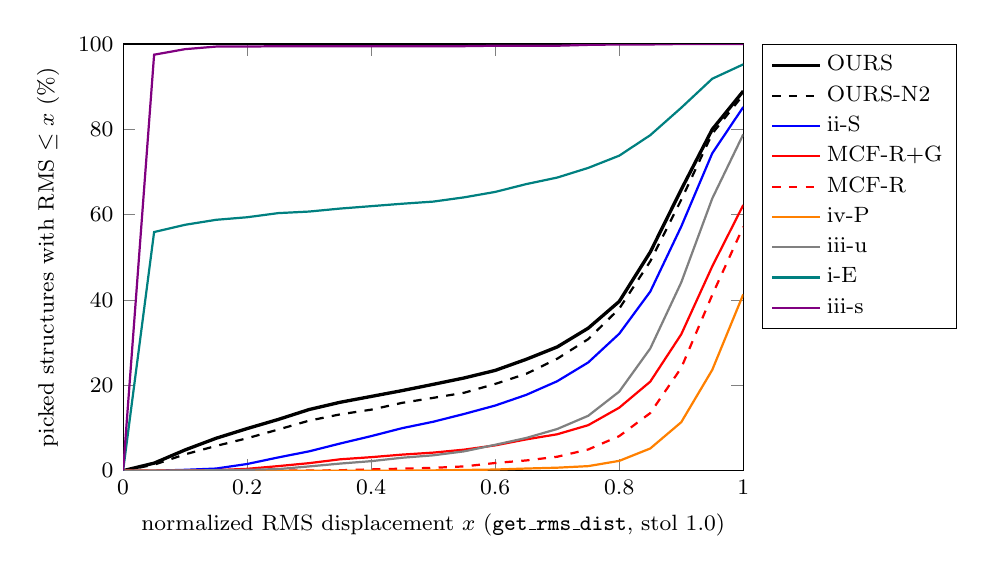
\begin{tikzpicture}
\begin{axis}[width=0.78\linewidth, height=7cm, xmin=0, xmax=1, ymin=0, ymax=100, xlabel={normalized RMS displacement $x$ (\texttt{get\_rms\_dist}, stol 1.0)}, ylabel={picked structures with RMS $\le x$ (\%)}, legend pos=outer north east, legend cell align=left, tick label style={font=\footnotesize}, label style={font=\footnotesize}, legend style={font=\footnotesize}]
\addplot[black, very thick] coordinates {(0,0.0000) (0.05,1.7667) (0.1,4.8667) (0.15,7.6000) (0.2,9.8667) (0.25,12.0000) (0.3,14.3333) (0.35,16.0333) (0.4,17.4000) (0.45,18.7667) (0.5,20.2333) (0.55,21.7333) (0.6,23.5000) (0.65,26.1000) (0.7,29.0000) (0.75,33.4000) (0.8,39.6667) (0.85,51.2333) (0.9,65.9000) (0.95,80.0000) (1,88.9667)};
\addlegendentry{OURS}
\addplot[black, dashed, thick] coordinates {(0,0.0000) (0.05,1.4000) (0.1,3.8333) (0.15,5.8000) (0.2,7.6000) (0.25,9.6333) (0.3,11.7333) (0.35,13.2000) (0.4,14.3000) (0.45,15.9000) (0.5,17.0667) (0.55,18.2667) (0.6,20.3333) (0.65,22.7000) (0.7,26.2333) (0.75,30.8333) (0.8,37.9667) (0.85,49.0667) (0.9,63.5000) (0.95,79.0000) (1,88.1000)};
\addlegendentry{OURS-N2}
\addplot[blue, thick] coordinates {(0,0.0000) (0.05,0.0000) (0.1,0.2000) (0.15,0.5000) (0.2,1.5667) (0.25,3.1000) (0.3,4.5333) (0.35,6.3667) (0.4,8.1000) (0.45,9.9667) (0.5,11.4667) (0.55,13.3000) (0.6,15.2667) (0.65,17.7667) (0.7,20.9667) (0.75,25.3667) (0.8,32.1000) (0.85,41.9667) (0.9,57.2333) (0.95,74.4000) (1,85.2333)};
\addlegendentry{ii-S}
\addplot[red, thick] coordinates {(0,0.0000) (0.05,0.0000) (0.1,0.0000) (0.15,0.1333) (0.2,0.4333) (0.25,1.0667) (0.3,1.7667) (0.35,2.6667) (0.4,3.1667) (0.45,3.7667) (0.5,4.2333) (0.55,4.9333) (0.6,5.9333) (0.65,7.3333) (0.7,8.5333) (0.75,10.6667) (0.8,14.7667) (0.85,20.8667) (0.9,31.9667) (0.95,47.9000) (1,62.2667)};
\addlegendentry{MCF-R+G}
\addplot[red, dashed, thick] coordinates {(0,0.0000) (0.05,0.0000) (0.1,0.0000) (0.15,0.0000) (0.2,0.0000) (0.25,0.0333) (0.3,0.0333) (0.35,0.1000) (0.4,0.3000) (0.45,0.4667) (0.5,0.6667) (0.55,1.0000) (0.6,1.8000) (0.65,2.4000) (0.7,3.2667) (0.75,4.9667) (0.8,8.1000) (0.85,13.5000) (0.9,24.1000) (0.95,41.2000) (1,57.1667)};
\addlegendentry{MCF-R}
\addplot[orange, thick] coordinates {(0,0.0000) (0.05,0.0000) (0.1,0.0000) (0.15,0.0000) (0.2,0.0000) (0.25,0.0000) (0.3,0.0000) (0.35,0.0000) (0.4,0.0000) (0.45,0.0000) (0.5,0.0667) (0.55,0.1667) (0.6,0.2667) (0.65,0.5000) (0.7,0.7000) (0.75,1.0667) (0.8,2.3000) (0.85,5.2000) (0.9,11.3667) (0.95,23.6333) (1,41.3333)};
\addlegendentry{iv-P}
\addplot[gray, thick] coordinates {(0,0.0000) (0.05,0.0000) (0.1,0.0333) (0.15,0.1000) (0.2,0.2000) (0.25,0.3667) (0.3,1.0000) (0.35,1.6667) (0.4,2.2333) (0.45,3.0333) (0.5,3.6000) (0.55,4.5333) (0.6,6.0667) (0.65,7.6667) (0.7,9.7667) (0.75,12.8667) (0.8,18.5333) (0.85,28.6333) (0.9,44.1333) (0.95,63.8000) (1,78.8333)};
\addlegendentry{iii-u}
\addplot[teal, thick] coordinates {(0,0.0000) (0.05,55.9333) (0.1,57.6333) (0.15,58.8000) (0.2,59.4000) (0.25,60.3667) (0.3,60.7333) (0.35,61.4333) (0.4,62.0000) (0.45,62.5667) (0.5,63.0667) (0.55,64.0667) (0.6,65.3333) (0.65,67.1667) (0.7,68.7000) (0.75,70.9667) (0.8,73.8333) (0.85,78.6333) (0.9,85.0667) (0.95,91.8667) (1,95.2333)};
\addlegendentry{i-E}
\addplot[violet, thick] coordinates {(0,0.0000) (0.05,97.5000) (0.1,98.8000) (0.15,99.4000) (0.2,99.4000) (0.25,99.5000) (0.3,99.5000) (0.35,99.5000) (0.4,99.5000) (0.45,99.5000) (0.5,99.5000) (0.55,99.5000) (0.6,99.6000) (0.65,99.6000) (0.7,99.6000) (0.75,99.8000) (0.8,99.9000) (0.85,99.9000) (0.9,100.0000) (0.95,100.0000) (1,100.0000)};
\addlegendentry{iii-s}
\end{axis}
\end{tikzpicture}

\caption{TEST-B ($n=\svN$): ECDF of the picked structure's normalised RMS displacement
(\texttt{get\_rms\_dist} at stol 1.0), mean over seeds, drawn through the stored 0.05 grid. A
curve that ends below 100\% at $x=1$ has picks that this matcher does not accept at all.
Values are those of Table~\ref{tab:si_ecdf}. Descriptive.}
\label{fig:si_ecdf}
\end{figure}
% src: generated/si_ecdf_fig_testB.tex <- results/n3/n3_results.json sets.testB.report.table1.<arm>.secondary.mcf10.rms_ecdf

\paragraph{Orientation error.} For the arms that output an asymmetric-unit orientation, the
protocol reports the geodesic angle between the picked $R_{\text{asym}}$ and the experimental
$R_0$, minimised over the molecule's proper point group (pymatgen's
\texttt{PointGroupAnalyzer}, tolerance 0.3~\AA; method parameters). Table~\ref{tab:si_geodesic}
gives its quantiles.

\begin{table}[htbp]
\caption{TEST-B ($n=\svN$): geodesic error (degrees) of the picked $R_{\text{asym}}$ to the
experimental $R_0$, minimised over the molecule's proper point group; quantiles per seed and
pooled over seeds ($q_{10}$ to $q_{90}$). For i-E and iii-s the picked orientation is the
FF$^\ast$-minimised one. Descriptive.}
\label{tab:si_geodesic}
\centering
\small
\begin{tabular}{@{}llccccc@{}}
\toprule
arm & seed & $q_{10}$ & $q_{25}$ & median & $q_{75}$ & $q_{90}$ \\
\midrule
\inputrows{generated/si_geodesic_testB.tex}
\bottomrule
\end{tabular}
\end{table}
% src: results/n3/n3_results.json sets.testB.report.table1.<arm>.geodesic_deg

\clearpage
% =====================================================================
\section{Ablations and descriptive arms}\label{si:ablations}
% =====================================================================
Three arms separate parts of the comparison and are reported without tests
(Table~\ref{tab:si_ablation}). \emph{ii-S} takes MolCrystalFlow's own sampled orientations from
the MCF-R+G checkpoints, maps each copy back to an asymmetric-unit orientation, expands each
exactly and keeps the lowest-LJ candidate, giving one candidate per draw (``MCF orientations
inside our exact space-group expansion''). \emph{iv-S} takes the identity copy's orientation from
the previous architecture (iv-P) as $R_{\text{asym}}$ and expands it exactly. \emph{i-E}
minimises all 16 OURS draws per seed with the universal interatomic potential FF$^\ast$ and picks
the lowest FF$^\ast$ energy; it separates the learned proposal from the energy model and is
scored in the H2 form (EXACT).

\begin{table}[htbp]
\caption{TEST-B ($n=\svN$), primary matcher: ablations and descriptive arms. picked@1 (\%) per
seed and seed mean $\pm$ s.d.; draw@1 and any@16 (\%); $\Delta$ = OURS $-$ arm (percentage
points), paired over crystals, with BCa 95\% CI and the two-stage interval that also resamples
seeds. Descriptive; no tests.}
\label{tab:si_ablation}
\centering
\scriptsize
\setlength{\tabcolsep}{3pt}
\begin{tabular}{@{}llcccccc@{}}
\toprule
arm & selector & per seed & mean $\pm$ s.d. & draw@1 & any@16 & $\Delta$ [BCa 95\% CI] & two-stage \\
\midrule
\inputrows{generated/si_ablation_testB.tex}
\bottomrule
\end{tabular}
\end{table}
% src: results/n3/n3_results.json sets.testB.report.table1.{ii-S,iv-S,i-E}

\paragraph{The ii-S decomposition.} Because ii-S and OURS share the exact expansion, the H1
component against MCF-R+G splits into two paired differences through the identity
\begin{equation}
\Delta(\text{OURS}-\text{MCF-R+G})=\Delta(\text{ii-S}-\text{MCF-R+G})+\Delta(\text{OURS}-\text{ii-S}),
\end{equation}
here \svDecTot{} = \svDecExp{} + \svDecLearn{} percentage points (pp), each term with its own
paired BCa interval (Table~\ref{tab:si_decomp}) and no $p$-value. Since the interval of
$\Delta(\text{OURS}-\text{ii-S})$ lies entirely above zero, the protocol's wording applies: our
learner adds \svDecLearn{} pp \svDecLearnCI{} over MolCrystalFlow's orientations inside the same
exact expansion (ablation estimate). The other term, \svDecExp{} pp \svDecExpCI, is the
difference made by expanding MolCrystalFlow's own orientations exactly.
% src: generated/si_decomp_testB.tex; tasks/n3_protocol.md:843-855 (Section 4, ii-S wording)

\begin{table}[htbp]
\caption{TEST-B ($n=\svN$): the ii-S decomposition of the H1 component against MCF-R+G.
$\Delta$ in pp, paired over crystals, with BCa 95\% CI, the two-stage seed interval and the
number of crystals with a nonzero paired difference. The two lower rows sum to the first.
Descriptive; no $p$-values.}
\label{tab:si_decomp}
\centering
\small
\begin{tabular}{@{}p{5.6cm}cccc@{}}
\toprule
difference & $\Delta$ (pp) & BCa 95\% CI & two-stage & nonzero \\
\midrule
\inputrows{generated/si_decomp_testB.tex}
\bottomrule
\end{tabular}
\end{table}
% src: results/n3/n3_results.json sets.testB.report.table1.MCF-R+G.delta_ours_minus_arm; .wording.ii_S_decomposition

\paragraph{Steric basin.} For continuity with our earlier work, the steric press (80 Adam steps
on the steric LJ energy; method parameters) is applied to the draws of OURS and of iii-p (P1),
and a hit is a match of the pressed draw to the pressed experimental structure
(Table~\ref{tab:si_steric}). Every reference completed the fixed 80-step press and was valid;
convergence was not assessed. The protocol prints our earlier DEV-TEST result beside it, as
history (DEV-TEST was used during development): \svGtwoContext.
% src: results/n3/n3_results.json sets.testB.report.steric_basin; tasks/n3_protocol.md:752-757
% src: reference press: sets.<set>.report.steric_basin.reference.ref_invalid_refcodes = [] and results/n3/private/draws/p1ref_s-1_<set>.pt (meta.steps 80, all valid), asserted in scripts/n3_si_tables.py; scripts/g2_asym_baselines.py:110-140 (fixed step count, no convergence flag)

\begin{table}[htbp]
\caption{TEST-B ($n=\svN$): steric basin (P1). picked@1 (\%) per seed and seed mean of each
arm's VALSEL-chosen P1 selector; $\Delta$ (pp) paired over crystals with BCa 95\% CI and the
two-stage interval. Descriptive; no tests.}
\label{tab:si_steric}
\centering
\footnotesize
\begin{tabular}{@{}p{3.4cm}lcccc@{}}
\toprule
 & selector & per seed & mean & $\Delta$ [BCa 95\% CI] & two-stage \\
\midrule
\inputrows{generated/si_steric_testB.tex}
\bottomrule
\end{tabular}
\end{table}
% src: results/n3/n3_results.json sets.testB.report.steric_basin

\paragraph{Descriptive contrasts around H2.} H2 was tested in its EXACT form, which scores the
search's minimised structure against the unrelaxed experimental one. Table~\ref{tab:si_h2desc}
gives the descriptive contrasts the protocol attaches to it: i-E against iii-s; OURS against
iii-s on the crystals whose experimental pose FF$^\ast$ holds (anchored), loses (drifted) or does
not converge (unresolved); on the crystals whose CSD refcode family is not in the potential's
OMC25 training data (OMC25 non-overlap); and in the secondary BASIN form, in which each arm's pick and the experimental
structure are both FF$^\ast$-minimised before matching. Table~\ref{tab:si_basin} gives the
BASIN-form rates. \svBasinUnconvN{} BASIN references (the FF$^\ast$-minimised experimental
structures) did not converge: \svBasinUnconv; none was invalid (\svBasinInvalid).
% src: results/n3/n3_results.json sets.testB.report.{i_e_vs_h2, wording.H2_by_ff_label, h2_omc25_nonoverlap, h2_basin_reference}, table1.iii-s.h2_basin_delta

\begin{table}[htbp]
\caption{TEST-B: descriptive contrasts around H2. $\Delta$ (pp) paired over the $n$ crystals of
each row, with BCa 95\% CI, the two-stage seed interval and the number of nonzero paired
differences. Rows with $n<30$ are too small to interpret. The H2 test itself is in the main
text. Descriptive; no tests.}
\label{tab:si_h2desc}
\centering
\footnotesize
\setlength{\tabcolsep}{3pt}
\begin{tabular}{@{}p{5.0cm}lrccr@{}}
\toprule
contrast & form & $n$ & $\Delta$ [BCa 95\% CI] & two-stage & nonzero \\
\midrule
\inputrows{generated/si_h2desc_testB.tex}
\bottomrule
\end{tabular}
\end{table}
% src: results/n3/n3_results.json sets.testB.report.{i_e_vs_h2, wording.H2_by_ff_label, h2_omc25_nonoverlap}, table1.iii-s.h2_basin_delta

\begin{table}[htbp]
\caption{TEST-B ($n=\svN$): picked@1 (\%) in the secondary BASIN form (the pick and the
experimental structure both FF$^\ast$-minimised before matching), per seed and seed mean, beside
the EXACT-form seed mean. iii-s is one deterministic run. Descriptive.}
\label{tab:si_basin}
\centering
\small
\begin{tabular}{@{}lccc@{}}
\toprule
arm & BASIN, per seed & BASIN, mean & EXACT, mean \\
\midrule
\inputrows{generated/si_basin_testB.tex}
\bottomrule
\end{tabular}
\end{table}
% src: results/n3/n3_results.json sets.testB.report.table1.<arm>.h2_basin_picked1_*

\clearpage
% =====================================================================
\section{The MolCrystalFlow fork, diagnostics and context arms}\label{si:mcfdiag}
% =====================================================================
\subsection{The fork}
MolCrystalFlow\cite{zeng2026molcrystalflow} (MCF) ran from its released code at commit
\svMcfBase{} in a fork limited to the patches the protocol permits (Table~\ref{tab:si_fork}).
The export gate (Gate F, Section~\ref{si:health}) confirmed the patched atom-type maps on every
exported set (\svForkSets).
% src: tasks/n3_protocol.md:372-393 (P1-P6), 1400-1403 (A3 item 5: P6 on); results/n3/gateF.json sets.<set>.p1_maps_patched

\begin{table}[htbp]
\caption{The MolCrystalFlow fork: every change to the released code (commit \svMcfBase), as the
protocol permits them. File and line references are to the released code.}
\label{tab:si_fork}
\centering
\small
\begin{tabular}{@{}lp{12.2cm}@{}}
\toprule
patch & change \\
\midrule
P1 & Four atom types added (Mg, As, Se, Te as indices 12--15) to the three atomic-number maps
(\texttt{data-preprocess/thurlemann23/common.py}, \texttt{molcrystalflow/data/utils.py},
\texttt{molcrystalflow/data/dataset.py}); inverses derived from them;
\texttt{model.bb\_embedder.num\_atom\_types = 16} in our configuration files. \\
P2 & Bug fix in \texttt{interpolant.corrupt\_batch}: with \texttt{trans.corrupt=False},
\texttt{b\_trans} is set to zeros (it was unbound). \\
P3 & MCF-R only: key \texttt{inference.gt\_lattice\_trans}. When on, the lattice and centroids
start at the truth, are reset to it after every Euler step and are used at final assembly;
rotations are untouched. \\
P4 & The GPU-selection calls return device 0. \\
P5 & \texttt{pl.seed\_everything(experiment.seed)} before the model is constructed. \\
P6 & Speed-ups: a vectorised symmetric SO(3) prior and a scatter-softmax attention pooling,
switched on after the equivalence checks on the cluster GPU (prior bit-identical; pooling outputs
and input gradients within $10^{-5}$ relative). \\
\bottomrule
\end{tabular}
\end{table}
% src: tasks/n3_protocol.md:372-393 (P1-P6), 1400-1403 (P6 on, A3); method details, no results

\subsection{Diagnostic (a): equivariance (PASS)}
On every selected MCF-R, MCF-R+G and MCF-A checkpoint, with the model and inputs in float64 on
the CPU, diagnostic (a) tests whether the network is equivariant to a common left rotation of
all molecular frames (10 VALSEL crystals $\times$ 3 random rotations; method parameters). The
tolerances are \svTolQ{} for the rotation-update vector, \svTolLat{} for the lattice output,
\svTolTr{} for the translation output and \svTolR{} for the predicted rotations; independent
per-copy rotations serve as controls and must exceed each statistic a hundredfold. The verdict
is \svDiagAVerdict{} on every checkpoint (Table~\ref{tab:si_diaga}), and the released
Thurlemann checkpoint, repeated for provenance, passes too.
% src: results/n3/n3_results.json mcf_diagnostic_a; tasks/n3_protocol.md:616-633

\begin{table}[htbp]
\caption{MCF diagnostic (a), per selected checkpoint: rotation-schedule rate $s_{uR}$ (and
$s_{uF}$ for MCF-A), verdict, the maximum deviations under a common rotation (rotation-update
vector $q$, lattice, translation, predicted rotations $R$) and the smallest control statistic
for each. Tolerances: $q$ \svTolQ, lattice \svTolLat, translation \svTolTr, $R$ \svTolR.}
\label{tab:si_diaga}
\centering
\scriptsize
\setlength{\tabcolsep}{2pt}
\begin{tabular}{@{}lllcccccccc@{}}
\toprule
 & & & \multicolumn{4}{c}{statistic} & \multicolumn{4}{c}{controls, minimum} \\
\cmidrule(lr){4-7}\cmidrule(lr){8-11}
checkpoint & knobs & verdict & $q$ & lattice & transl. & $R$ & $q$ & lattice & transl. & $R$ \\
\midrule
\inputrows{generated/si_diaga_stats.tex}
\bottomrule
\end{tabular}
\end{table}
% src: results/n3/n3_results.json mcf_diagnostic_a.per_checkpoint.<ckpt>.{knobs,verdict,statistics,controls_min,tolerances}

\paragraph{Why (b)--(d) are approximate.} The relative-rotation azimuth feature of MCF has a
branch cut, and the exact C$_2$-conjugate copies of every symmetric-prior draw sit on it at
$t=0$ (amendment A2). The 50-step sampler deviation, the largest departure from equivariance of
the final rotations when the full sampler is run from the same prior draw and from its rotated
copy, therefore exceeds $10^{-3}$ on all
\svDiagAApproxN{} selected checkpoints (\svDiagAApprox; Table~\ref{tab:si_diaga2}), and by the
rule of A2 the outputs of diagnostics (b)--(d) are labelled approximate. At the corrupted batch
state the selected checkpoints give the harness verdict HARNESS\_CHECK (reported, not gated),
with edges on the branch cut; the Thurlemann checkpoint, whose prior draw has none on the cut,
passes there.
% src: results/n3/n3_results.json mcf_diagnostic_a.{approximate_checkpoints, approximate_rule}, per_checkpoint.<ckpt>.{sampler_deviation, corrupt_batch_state}

\begin{table}[htbp]
\caption{MCF diagnostic (a), sampler and harness fields (reported, not gated): the 50-step
sampler deviation of the predicted rotations in the native float32 run and in a float64
replica, whether the float32 deviation exceeds $10^{-3}$ (the A2 rule that labels (b)--(d)
approximate), the verdict at the corrupted batch state, and the edges of that state on the
azimuth branch cut.}
\label{tab:si_diaga2}
\centering
\small
\begin{tabular}{@{}lccccc@{}}
\toprule
 & \multicolumn{3}{c}{50-step sampler deviation} & \multicolumn{2}{c}{corrupted batch} \\
\cmidrule(lr){2-4}\cmidrule(lr){5-6}
checkpoint & float32 & float64 & $>10^{-3}$ & verdict & on cut/edges \\
\midrule
\inputrows{generated/si_diaga_sampler.tex}
\bottomrule
\end{tabular}
\end{table}
% src: results/n3/n3_results.json mcf_diagnostic_a.per_checkpoint.<ckpt>.{sampler_deviation, sampler_deviation_threshold_1e-3, corrupt_batch_state}

\subsection{Diagnostics (b)--(d) (approximate)}
\paragraph{(b) Perfect-model ceiling (oracle, approximate).} For each crystal, $c_i$ is the Haar
fraction of MCF's invariance group whose common rotation of the true molecular frames still
matches the experimental structure: a \svDiagBGrid$^\circ$ grid walked at \svDiagBWalk$^\circ$ to
the window edges for $z_\mathrm{MCF}=2$, the matching fraction of the D$_2$ elements for
$z_\mathrm{MCF}\ge3$, and the iii-u Haar floor for $z_\mathrm{MCF}=1$. Its mean is a ceiling on
MCF's draw@1, and $1-(1-c_i)^{16}$ on its any@16 (Table~\ref{tab:si_diagb}). The draw@1 ceiling
does not bound LJ-picked@1 (results file: ``\svDiagBNote''), because a selector can pick
better than a random draw.

\begin{table}[htbp]
\caption{TEST-B: MCF diagnostic (b), perfect-model ceiling (oracle item, approximate), per
matcher and $z_\mathrm{MCF}$ (molecules in the exported MCF cell): mean $c_i$ (draw@1 ceiling,
\%) and mean $1-(1-c_i)^{16}$ (any@16 ceiling, \%). For $z_\mathrm{MCF}=1$ the value is the
Haar floor, as labelled. The draw@1 ceiling does not bound LJ-picked@1. An oracle diagnostic
using experimental truth.}
\label{tab:si_diagb}
\centering
\small
\begin{tabular}{@{}lcrccl@{}}
\toprule
matcher & $z_\mathrm{MCF}$ & $n$ & draw@1 ceiling & any@16 ceiling & label \\
\midrule
\inputrows{generated/si_diagb_testB.tex}
\bottomrule
\end{tabular}
\end{table}
% src: results/n3/n3_results.json sets.testB.mcf_diagnostics.b.summary

\paragraph{(c) Oracle-aligned score (oracle, approximate).} Each MCF-R draw is first moved by the
element of MCF's invariance group that best aligns its frames with the true ones, and then
matched (Table~\ref{tab:si_diagc}). The alignment uses the true frames, so this is an oracle
item: an oracle diagnostic using experimental truth. It is not computed for the \svDiagCZoneN{} crystals with $z_\mathrm{MCF}=1$, where
it is exact by construction.

\begin{table}[htbp]
\caption{TEST-B: MCF diagnostic (c), oracle-aligned MCF-R scores (oracle item, approximate; LJ
selector): draw@1 per seed and mean, any@16 (mean) and picked@1 per seed and mean, all in \%.
An oracle diagnostic using experimental truth.}
\label{tab:si_diagc}
\centering
\footnotesize
\setlength{\tabcolsep}{3pt}
\begin{tabular}{@{}lcrccccc@{}}
\toprule
matcher & $z_\mathrm{MCF}$ & $n$ & draw@1, per seed & draw@1 & any@16 & picked@1, per seed & picked@1 \\
\midrule
\inputrows{generated/si_diagc_testB.tex}
\bottomrule
\end{tabular}
\end{table}
% src: results/n3/n3_results.json sets.testB.mcf_diagnostics.c.matchers

\paragraph{(d) Consistency (approximate).} MCF-R's unaligned draw@1 must not exceed the (b)
ceiling beyond its bootstrap interval; an exceedance would mean that (b) is wrong. No stratum
exceeds it under any matcher (consistent: \svDiagDConsistent; Table~\ref{tab:si_diagd}).

\begin{table}[htbp]
\caption{TEST-B: MCF diagnostic (d), consistency (approximate): MCF-R's unaligned draw@1 (\%)
with its 95\% bootstrap interval, the (b) draw@1 ceiling (\%), and whether the draw@1 exceeds the
ceiling.}
\label{tab:si_diagd}
\centering
\small
\begin{tabular}{@{}lcrcccc@{}}
\toprule
matcher & $z_\mathrm{MCF}$ & $n$ & draw@1 & 95\% interval & ceiling & exceeds \\
\midrule
\inputrows{generated/si_diagd_testB.tex}
\bottomrule
\end{tabular}
\end{table}
% src: results/n3/n3_results.json sets.testB.mcf_diagnostics.d

\subsection{Context arms: MCF-A and the prior floor}
MCF-A is MolCrystalFlow trained and sampled with its released joint objective, generating the
lattice and centroids as well as the orientations. It receives less information than every
other arm and is context only: it never enters H1--H3. Its prior floor samples the refit
lattice prior, uniform centroids and symmetric-prior rotations. The protocol reports both under
MCF's native rule at three tolerances as well as the primary matcher (Table~\ref{tab:si_mcfa}).
The protocol also asks for the number of MCF-A draws whose generated cell has an interplanar
spacing below 2.5~\AA{} (the smallest height $V/|\mathbf{a}_j\times\mathbf{a}_k|$ of the cell as
generated; these draws receive $e_\mathrm{LJ}=+\infty$). On TEST-B they are \svSpacingMcfA{} of
the \svSpacingDraws{} draws of seeds 0, 1 and 2, and \svSpacingMcfAFloor{} of the prior
floor's; on DEV-TEST, \svSpacingMcfADev{} of \svSpacingDrawsDev{}, and \svSpacingMcfAFloorDev{}.
% src: results/n3/n3_results.json sets.testB.report.table1.{MCF-A,MCF-A-floor}; tasks/n3_protocol.md:598-613 (spacing count requested), 1198-1199 (A2 item 5: height definition)
% src: spacing counts: generated/si_numbers.tex svSpacing* <- results/n3/private/draws/<MCF-A and floor bundles>.pt meta.lj_counts.spacing_inf (scripts/n3_mcf_run.py:852-857; scripts/n3_mcf_lib.py:47,352-359)

\begin{table}[htbp]
\caption{TEST-B ($n=\svN$): context table, MCF-A and its prior floor. picked@1 (\%) per seed
and for the ensemble (3-model ensemble, 48 draws) under the primary matcher and MCF's rule at
stol 0.5, 0.8 and 1.0; draw@1 and any@16 (\%) are recorded for the primary matcher only.
Context only; no tests.}
\label{tab:si_mcfa}
\centering
\footnotesize
\setlength{\tabcolsep}{3pt}
\begin{tabular}{@{}lllcccc@{}}
\toprule
arm & selector & matcher & picked@1, per seed & ensemble & draw@1 & any@16 \\
\midrule
\inputrows{generated/si_mcfa_testB.tex}
\bottomrule
\end{tabular}
\end{table}
% src: results/n3/n3_results.json sets.testB.report.table1.{MCF-A,MCF-A-floor}

\clearpage
% =====================================================================
\section{Strata in full (main-text Table 5)}\label{si:strata}
% =====================================================================
Table~5 of the main text gives seed-mean picked@1 by stratum. Tables~\ref{tab:si_strata} and
\ref{tab:si_strata_sens} give, for every stratum, level and arm, the number of crystals picked
correctly in each seed ($k$, s0 / s1 / s2), the Wilson 95\% interval of each seed's rate, and the
ensemble count and its Wilson interval. The random floor's $k$ is fractional because RANDOM is
scored as its exact expectation. Levels with $n<30$ are marked ``too small to interpret''. Each
$z_\mathrm{MCF}$ level carries MCF's diagnostic-(b) ceiling under the primary matcher, labelled
oracle and approximate; as above, this draw@1 ceiling does not bound LJ-picked@1. The FF$^\ast$
truth label is reported for the H2 pair only (OURS, OURS-N2 and iii-s). The sensitivity strata
(Table~\ref{tab:si_strata_sens}) repeat the three handedness strata. A conformer is chiral
(geometrically, as a rigid body) when its refined mirror RMSD exceeds 0.3~\AA; the refined
mirror RMSD is the minimum of a proper-rotation Kabsch fit over the first 200
element-matched graph automorphisms and an element-blocked Hungarian ICP (30 iterations, 5
deterministic starts). A cell is mixed-handedness when the conformer is chiral and the space
group has an improper operation, and improper-achiral when it has an improper operation but
the conformer is not chiral. The sensitivity rows use the refined mirror-RMSD
definition at thresholds of 0.1 and 0.5~\AA{} and under the parser-capped definition (200
automorphisms) at 0.3~\AA{} (method parameters; the primary definition is refined, 0.3~\AA).
All rows are descriptive, with no tests.
% src: tasks/n3_protocol.md:336-358 (Section 2.6)

\begingroup
\singlespacing
\scriptsize
\setlength{\tabcolsep}{3pt}
\begin{longtable}{@{}lcccccc@{}}
\caption{TEST-B ($n=\svN$), primary matcher: every stratum of main-text Table~5 in full. $k$: crystals
picked correctly per seed (iii-s: one run); Wilson 95\% intervals (\%) per seed and for the
ensemble (3-model ensemble, 48 draws). Descriptive; no tests.}
\label{tab:si_strata}\\
\toprule
arm & $k$ (s0 / s1 / s2) & Wilson s0 & Wilson s1 & Wilson s2 & $k$, ensemble & Wilson, ensemble \\
\midrule
\endfirsthead
\multicolumn{7}{@{}l}{Table~\thetable{} (continued)} \\
\toprule
arm & $k$ (s0 / s1 / s2) & Wilson s0 & Wilson s1 & Wilson s2 & $k$, ensemble & Wilson, ensemble \\
\midrule
\endhead
\bottomrule
\endfoot
\inputrows{generated/si_strata_testB.tex}
\end{longtable}
\endgroup
% src: results/n3/n3_results.json sets.testB.report.table2 (main strata); sets.testB.mcf_diagnostics.b.summary.primary

\begingroup
\singlespacing
\scriptsize
\setlength{\tabcolsep}{3pt}
\begin{longtable}{@{}lcccccc@{}}
\caption{TEST-B ($n=\svN$), primary matcher: sensitivity strata of the handedness definitions,
in the layout of Table~\ref{tab:si_strata}. Descriptive; no tests.}
\label{tab:si_strata_sens}\\
\toprule
arm & $k$ (s0 / s1 / s2) & Wilson s0 & Wilson s1 & Wilson s2 & $k$, ensemble & Wilson, ensemble \\
\midrule
\endfirsthead
\multicolumn{7}{@{}l}{Table~\thetable{} (continued)} \\
\toprule
arm & $k$ (s0 / s1 / s2) & Wilson s0 & Wilson s1 & Wilson s2 & $k$, ensemble & Wilson, ensemble \\
\midrule
\endhead
\bottomrule
\endfoot
\inputrows{generated/si_strata_sens_testB.tex}
\end{longtable}
\endgroup
% src: results/n3/n3_results.json sets.testB.report.table2 (sensitivity.* strata)

\clearpage
% =====================================================================
\section{Representability in full (main-text Table 2)}\label{si:tabler}
% =====================================================================
Table~R counts the crystals whose \emph{true} structure each representation can emit, before
any sampling. The frozen wording of the protocol (its Section~5), with the TEST-B counts, reads:
``\svTRText'' The MolCrystalFlow paper describes a mixed-handedness crystal structure
prediction scenario whose code is not released at the commit we used (\svMcfBase).

\paragraph{(a) Exact expansion.} Column (a), exact expansion with the full space-group operations
(OURS and the classical arms), represents every TEST-B crystal by construction, because build
step~2 keeps only crystals whose expansion reproduces them: it removed the crystals that are
not $Z'=1$ general-position and those whose expansion orbit failed (Table~\ref{tab:si_build}).
On DEV-TEST, column (a) is computed rather than true by construction, and it covers every
crystal.
No representability claim is made against MolCrystalFlow's per-copy representation, column (b),
which also covers the $Z'>1$ and special-position crystals our design excludes (\svDevNotEligible{}
of the \svDevOThree{} parsed crystals of the development corpus).

\paragraph{(c) The released MCF driver: the homochiral approximant.} The released MCF crystal
structure prediction driver uses one conformer and one handedness for all copies. Column (c)
is the lowest-RMSD homochiral approximant found: the true lattice and centroids, with each copy
made by an improper operation replaced by the lowest-RMSD proper rotation onto its mirror image
found by element-blocked ICP. A multi-start search gives no global-optimality certificate, and
minimising per-molecule RMSD does not optimise the matcher's criterion, so a non-match shows
that this approximant fails, not that every homochiral cell would. The protocol fixed 16 starts (the four sign-diagonal rotations and twelve
seeded random rotations); amendment A2 added the best automorphism rotation as a 17th start,
and the 16-start column is reported beside it. The extra start lowered the optimum for
\svTRAutoImproved{} TEST-B crystals (largest RMSD gain \svTRMaxGain~\AA), and the two columns
differ in outcome for \svTRChangedHalf{} crystals at stol 0.5 and for \svTRChangedPrimary{}
under the primary matcher: the approximant matches \svTRQ/\svTRMixed{} mixed-handedness crystals at
stol 0.5 with 17 starts and \svTRQSixteen/\svTRMixed{} with the 16 frozen starts
(Table~\ref{tab:si_tabler_c}). With the 16 frozen starts alone the frozen sentence reads:
``\svTRTextSixteen''

\paragraph{(d) The legacy det$+$1 pipeline: keep flag and oracle rebuild.} Column (d) counts
the crystals the legacy pipeline kept (the part-file keep flag); the frozen sentence uses this
count (\svTRN{} not representable, \svTRM{} of them centrosymmetric). For the kept crystals,
\texttt{n3\_legacy\_oracle.py} rebuilds the structure with a fresh registry and matches it to
the CIF; that rebuild match is reported separately (``oracle'' columns of
Table~\ref{tab:si_tabler_abd}). Counting kept crystals whose rebuild misses the primary
matcher as unrepresentable as well gives \svTRNOracle{} (\svTRMOracle{} centrosymmetric). Every
Table~R job finished within its \svTRTimeout-s limit; timeouts, deterministic failures, errors
and missing rows sum to \svTRBad{} on TEST-B and \svTRBadDev{} on DEV-TEST.
% src: results/n3/table_r_testB.json, table_r_devtest.json (wording, c_diagnostics, rows, corpus_context, timing_s); tasks/n3_protocol.md:876-910

\begin{table}[htbp]
\caption{Table~R in full, columns (a), (b) and (d): crystals whose true structure the
representation can emit, under the primary matcher and MCF's rule at stol 0.5 and 0.8. (a) exact
expansion with the full operations; (b) MCF's per-copy representation; (d) the legacy det$+$1
pipeline: the part-file keep flag, and the oracle rebuild of the kept crystals. DEV-TEST rows:
used during development, not confirmatory.}
\label{tab:si_tabler_abd}
\centering
\footnotesize
\setlength{\tabcolsep}{3pt}
\begin{tabular}{@{}lrcccccccccc@{}}
\toprule
 & & \multicolumn{3}{c}{(a) exact expansion} & \multicolumn{3}{c}{(b) MCF per copy} & \multicolumn{4}{c}{(d) legacy det$+$1} \\
\cmidrule(lr){3-5}\cmidrule(lr){6-8}\cmidrule(lr){9-12}
 & & & & & & & & keep & \multicolumn{3}{c}{oracle rebuild} \\
\cmidrule(lr){10-12}
row & $n$ & primary & 0.5 & 0.8 & primary & 0.5 & 0.8 & flag & primary & 0.5 & 0.8 \\
\midrule
\inputrows{generated/si_tabler_abd.tex}
\bottomrule
\end{tabular}
\end{table}
% src: results/n3/table_r_testB.json, table_r_devtest.json rows.<row>.{a,b,d}

\begin{table}[htbp]
\caption{Table~R in full, column (c): the lowest-RMSD homochiral approximant found for the released MCF
driver, with 17 starts (16 frozen plus the best automorphism rotation, amendment A2) and with
the 16 frozen starts alone, under the primary matcher and MCF's rule at stol 0.5 and 0.8.
``no improper op'': crystals without an improper operation, which (c) represents as (a) does;
``multiple optima'': crystals with tied distinct optima, scored as a match if any matches.
DEV-TEST rows: used during development, not confirmatory.}
\label{tab:si_tabler_c}
\centering
\footnotesize
\setlength{\tabcolsep}{3pt}
\begin{tabular}{@{}lrccccccrr@{}}
\toprule
 & & \multicolumn{3}{c}{(c), 17 starts} & \multicolumn{3}{c}{(c), 16 frozen starts} & & \\
\cmidrule(lr){3-5}\cmidrule(lr){6-8}
row & $n$ & primary & 0.5 & 0.8 & primary & 0.5 & 0.8 & no improper op & multiple optima \\
\midrule
\inputrows{generated/si_tabler_c.tex}
\bottomrule
\end{tabular}
\end{table}
% src: results/n3/table_r_testB.json, table_r_devtest.json rows.<row>.{c,c_frozen16}

\begin{table}[htbp]
\caption{Construction of TEST-B and SEL from the pool of CIFs: crystals remaining after each
build step, and the removals of build steps 2 and 3. Build step 2 is the eligibility filter
behind column (a).}
\label{tab:si_build}
\centering
\small
\begin{tabular}{@{}lr@{}}
\toprule
step & crystals \\
\midrule
\inputrows{generated/si_build.tex}
\bottomrule
\end{tabular}
\end{table}
% src: results/n3/table_r_testB.json corpus_context.pool.build_counts, build_step2

\clearpage
% =====================================================================
\section{DEV-TEST}\label{si:devtest}
% =====================================================================
DEV-TEST holds \svNDev{} crystals that were used during development (disclosures (a)--(e),
Section~\ref{si:disclosures}). Every arm that ran on TEST-B ran on it with the same frozen
configuration, and its rows form a secondary continuity record. Every table in this section is
labelled ``used during development, not confirmatory''; none carries a test, and the frozen
report computes no hypothesis family on DEV-TEST. The OURS and OURS-N2 rows reuse the draws
stored during development, re-matched from their rotations.
% src: results/n3/n3_results.json sets.devtest.{role,families}; tasks/n3_protocol.md:332-334 (Section 2.5)

\begin{table}[htbp]
\caption{\devlabel, primary matcher: every arm. picked@1 (\%) per seed and seed mean $\pm$
s.d.; $\Delta$ = OURS $-$ arm (pp, paired over crystals) with BCa 95\% CI and the two-stage
interval; draw@1 and any@16 (\%). Rows below the rule: ablations, descriptive and context arms.
No tests.}
\label{tab:si_dev_t1}
\centering
\scriptsize
\setlength{\tabcolsep}{2.5pt}
\begin{tabular}{@{}llcccccc@{}}
\toprule
arm & selector & per seed & mean $\pm$ s.d. & $\Delta$ [BCa 95\% CI] & two-stage & draw@1 & any@16 \\
\midrule
\inputrows{generated/si_t1_devtest.tex}
\bottomrule
\end{tabular}
\end{table}
% src: results/n3/n3_results.json sets.devtest.report.table1

\begin{table}[htbp]
\caption{\devlabel: secondary matchers, in the layout of Table~\ref{tab:si_secondary}. No
tests.}
\label{tab:si_dev_secondary}
\centering
\footnotesize
\setlength{\tabcolsep}{3pt}
\begin{tabular}{@{}llcccc@{}}
\toprule
 & & \multicolumn{2}{c}{stol 0.5} & \multicolumn{2}{c}{stol 0.8} \\
\cmidrule(lr){3-4}\cmidrule(lr){5-6}
arm & selector & per seed & ens. & per seed & ens. \\
\midrule
\inputrows{generated/si_secondary_devtest.tex}
\bottomrule
\end{tabular}
\end{table}
% src: results/n3/n3_results.json sets.devtest.report.table1.<arm>.secondary

\begin{table}[htbp]
\caption{\devlabel: ensembles and any-of-all-draws, in the layout of
Table~\ref{tab:si_ensemble}. No tests.}
\label{tab:si_dev_ensemble}
\centering
\footnotesize
\setlength{\tabcolsep}{3pt}
\begin{tabular}{@{}llcccc@{}}
\toprule
arm & ensemble & picked@1 & ensemble picked@1 & any@16 & any, all draws \\
\midrule
\inputrows{generated/si_ensemble_devtest.tex}
\bottomrule
\end{tabular}
\end{table}
% src: results/n3/n3_results.json sets.devtest.report.table1.<arm>.{ensemble_*,any_all_pct}

\begin{table}[htbp]
\caption{\devlabel: ECDF of the picked structure's normalised RMS displacement, in the layout and
with the notes of Table~\ref{tab:si_ecdf}. No tests.}
\label{tab:si_dev_ecdf}
\centering
\footnotesize
\begin{tabular}{@{}lcccccc@{}}
\toprule
arm & $x=0.1$ & 0.2 & 0.3 & 0.5 & 0.8 & 1.0 \\
\midrule
\inputrows{generated/si_ecdf_devtest.tex}
\bottomrule
\end{tabular}
\end{table}
% src: results/n3/n3_results.json sets.devtest.report.table1.<arm>.secondary.mcf10.rms_ecdf

\begin{table}[htbp]
\caption{\devlabel: geodesic orientation error (degrees), in the layout of
Table~\ref{tab:si_geodesic}.}
\label{tab:si_dev_geodesic}
\centering
\small
\begin{tabular}{@{}llccccc@{}}
\toprule
arm & seed & $q_{10}$ & $q_{25}$ & median & $q_{75}$ & $q_{90}$ \\
\midrule
\inputrows{generated/si_geodesic_devtest.tex}
\bottomrule
\end{tabular}
\end{table}
% src: results/n3/n3_results.json sets.devtest.report.table1.<arm>.geodesic_deg

\begin{table}[htbp]
\caption{\devlabel: ablations and descriptive arms, in the layout of
Table~\ref{tab:si_ablation}. No tests.}
\label{tab:si_dev_ablation}
\centering
\scriptsize
\setlength{\tabcolsep}{3pt}
\begin{tabular}{@{}llcccccc@{}}
\toprule
arm & selector & per seed & mean $\pm$ s.d. & draw@1 & any@16 & $\Delta$ [BCa 95\% CI] & two-stage \\
\midrule
\inputrows{generated/si_ablation_devtest.tex}
\bottomrule
\end{tabular}
\end{table}
% src: results/n3/n3_results.json sets.devtest.report.table1.{ii-S,iv-S,i-E}

\begin{table}[htbp]
\caption{\devlabel: steric basin (P1), in the layout of Table~\ref{tab:si_steric}. Every
reference completed the fixed 80-step press and was valid; convergence was not assessed. No
tests.}
\label{tab:si_dev_steric}
\centering
\footnotesize
\begin{tabular}{@{}p{3.4cm}lcccc@{}}
\toprule
 & selector & per seed & mean & $\Delta$ [BCa 95\% CI] & two-stage \\
\midrule
\inputrows{generated/si_steric_devtest.tex}
\bottomrule
\end{tabular}
\end{table}
% src: results/n3/n3_results.json sets.devtest.report.steric_basin

\begin{table}[htbp]
\caption{\devlabel: descriptive contrasts around H2, in the layout of
Table~\ref{tab:si_h2desc} (the FF$^\ast$-label split is computed for TEST-B only). Unconverged
BASIN references: \svBasinUnconvNDev{} (\svBasinUnconvDev). No tests.}
\label{tab:si_dev_h2desc}
\centering
\footnotesize
\setlength{\tabcolsep}{3pt}
\begin{tabular}{@{}p{5.0cm}lrccr@{}}
\toprule
contrast & form & $n$ & $\Delta$ [BCa 95\% CI] & two-stage & nonzero \\
\midrule
\inputrows{generated/si_h2desc_devtest.tex}
\bottomrule
\end{tabular}
\end{table}
% src: results/n3/n3_results.json sets.devtest.report.{i_e_vs_h2, h2_omc25_nonoverlap, h2_basin_reference}, table1.iii-s.h2_basin_delta

\begin{table}[htbp]
\caption{\devlabel: BASIN-form picked@1 (\%), in the layout of Table~\ref{tab:si_basin}.}
\label{tab:si_dev_basin}
\centering
\small
\begin{tabular}{@{}lccc@{}}
\toprule
arm & BASIN, per seed & BASIN, mean & EXACT, mean \\
\midrule
\inputrows{generated/si_basin_devtest.tex}
\bottomrule
\end{tabular}
\end{table}
% src: results/n3/n3_results.json sets.devtest.report.table1.<arm>.h2_basin_picked1_*

\begingroup
\singlespacing
\scriptsize
\setlength{\tabcolsep}{2.5pt}
\begin{longtable}{@{}p{3.1cm}lrccccccccc@{}}
\caption{\devlabel: seed-mean picked@1 (\%) by stratum for the Table~1 arms (the layout of
Table~5 of the main text), including the sensitivity strata. $^{*}$Fewer than 30 crystals: too
small to interpret. The FF$^\ast$ truth label is reported for the H2 pair only. No tests.}
\label{tab:si_dev_strata}\\
\toprule
stratum & & $n$ & floor & iii-u & iii-p & iii-s & iv-P & MCF-R & MCF-R+G & OURS & OURS-N2 \\
\midrule
\endfirsthead
\multicolumn{12}{@{}l}{Table~\thetable{} (continued)} \\
\toprule
stratum & & $n$ & floor & iii-u & iii-p & iii-s & iv-P & MCF-R & MCF-R+G & OURS & OURS-N2 \\
\midrule
\endhead
\bottomrule
\endfoot
\inputrows{generated/si_strata_devtest.tex}
\end{longtable}
\endgroup
% src: results/n3/n3_results.json sets.devtest.report.table2

\begin{table}[htbp]
\caption{\devlabel: MCF diagnostic (b), perfect-model ceiling (oracle item, approximate), in the
layout of Table~\ref{tab:si_diagb}. DEV-TEST has no $z_\mathrm{MCF}=1$ crystal. The draw@1
ceiling does not bound LJ-picked@1. Non-confirmatory diagnostic.}
\label{tab:si_dev_diagb}
\centering
\small
\begin{tabular}{@{}lcrccl@{}}
\toprule
matcher & $z_\mathrm{MCF}$ & $n$ & draw@1 ceiling & any@16 ceiling & label \\
\midrule
\inputrows{generated/si_diagb_devtest.tex}
\bottomrule
\end{tabular}
\end{table}
% src: results/n3/n3_results.json sets.devtest.mcf_diagnostics.b.summary

\begin{table}[htbp]
\caption{\devlabel: MCF diagnostic (c), oracle-aligned MCF-R scores (oracle item, approximate),
in the layout of Table~\ref{tab:si_diagc}. Non-confirmatory diagnostic.}
\label{tab:si_dev_diagc}
\centering
\footnotesize
\setlength{\tabcolsep}{3pt}
\begin{tabular}{@{}lcrccccc@{}}
\toprule
matcher & $z_\mathrm{MCF}$ & $n$ & draw@1, per seed & draw@1 & any@16 & picked@1, per seed & picked@1 \\
\midrule
\inputrows{generated/si_diagc_devtest.tex}
\bottomrule
\end{tabular}
\end{table}
% src: results/n3/n3_results.json sets.devtest.mcf_diagnostics.c.matchers

\begin{table}[htbp]
\caption{\devlabel: MCF diagnostic (d), consistency (approximate), in the layout of
Table~\ref{tab:si_diagd}; consistent: \svDiagDConsistentDev.}
\label{tab:si_dev_diagd}
\centering
\small
\begin{tabular}{@{}lcrcccc@{}}
\toprule
matcher & $z_\mathrm{MCF}$ & $n$ & draw@1 & 95\% interval & ceiling & exceeds \\
\midrule
\inputrows{generated/si_diagd_devtest.tex}
\bottomrule
\end{tabular}
\end{table}
% src: results/n3/n3_results.json sets.devtest.mcf_diagnostics.d

\begin{table}[htbp]
\caption{\devlabel: context table, MCF-A and its prior floor, in the layout of
Table~\ref{tab:si_mcfa}. Context only; no tests.}
\label{tab:si_dev_mcfa}
\centering
\footnotesize
\setlength{\tabcolsep}{3pt}
\begin{tabular}{@{}lllcccc@{}}
\toprule
arm & selector & matcher & picked@1, per seed & ensemble & draw@1 & any@16 \\
\midrule
\inputrows{generated/si_mcfa_devtest.tex}
\bottomrule
\end{tabular}
\end{table}
% src: results/n3/n3_results.json sets.devtest.report.table1.{MCF-A,MCF-A-floor}

\clearpage
% =====================================================================
\section{The VALSEL selection grids}\label{si:valsel}
% =====================================================================
Every choice the protocol leaves open was made on VALSEL (VAL then SEL, \svValselN{} crystals),
before any TEST-B or DEV-TEST input reached the cluster, and frozen in the step-6 selection
record (SHA-256 \svSelSha, commit \svSelCommit). Table~\ref{tab:si_sel_summary} lists every
frozen choice and the criterion that decided it; Tables~\ref{tab:si_sel_a} and
\ref{tab:si_sel_b} give the full grids. Counts are summed over the three seeds (method
parameter): ``hits'' are seed-summed VALSEL picks that match under the primary matcher, draw@1
is the seed-summed expected number of matches of a random draw, and any@16 the seed-summed
number of crystals with at least one matching draw.

\paragraph{How ties were broken.} Each grid was decided by its first criterion unless candidates
tied on it, and ties went down the preregistered order printed with each grid. For selectors the
last key is the preference LJ $>$ RESID $>$ MODE@$r$ (smaller $r$ first) $>$ RANDOM; it decided
iii-u (LJ, MODE@0.25 and MODE@0.5 tied on hits) and iv-P Stage~A (no selector scored a hit). The
MCF-R+G rate $s_{uR}$ was decided by draw@1 after two cells tied on hits. For checkpoints the
order is VALSEL picked@1, then draw@1, then any@16, and the final tie-break is the lower
fixed-draw VAL loss (for MCF-A Stage~1: any-of-10 at stol 1.0, then at stol 0.8, then MCF's
logged validation loss). The final tie-break decided MCF-R seeds 0 and 1, MCF-R+G seed 1 and all
three iv-P seeds; in each of those cases the candidates were tied on every VALSEL criterion. For
the MCF arms the checkpoint labelled ``last'' is the latest-epoch top-3 checkpoint, not
final-epoch weights (Section~\ref{si:mcfckpt}).
% src: results/n3/n3_selection.json valsel_cell_scores.<grid>.{stage_a,stage_b}.{tie,decided_by}; tasks/n3_protocol.md:251-276,1530-1541

\begingroup
\singlespacing
\footnotesize
\begin{longtable}{@{}p{4.4cm}p{6.6cm}p{4.2cm}@{}}
\caption{Every frozen VALSEL choice and what decided it (step-6 selection record).}
\label{tab:si_sel_summary}\\
\toprule
choice & frozen value & decided by \\
\midrule
\endfirsthead
\toprule
choice & frozen value & decided by \\
\midrule
\endhead
\bottomrule
\endfoot
\inputrows{generated/si_sel_summary.tex}
\end{longtable}
\endgroup
% src: results/n3/n3_selection.json frozen, valsel_cell_scores

\begingroup
\singlespacing
\scriptsize
\setlength{\tabcolsep}{3pt}
\begin{longtable}{@{}llccccl@{}}
\caption{VALSEL grids for selectors and sampler settings (Stage~A and single-stage grids),
\svValselN{} crystals, counts summed over three seeds. The score column is the grid's first
criterion (named in each header): seed-summed hits, any-of-10 at stol 1.0 (MCF-A Stage~2) or
picked@1 at stol 1.0 (MCF-A Stage~3). $s_{uR}$, $s_{uF}$: MCF's rotation- and frame-schedule
rates; ``pref.'': the cell preferred on ties.}
\label{tab:si_sel_a}\\
\toprule
cell & selector & draw@1 & any@16 & score & per seed & \\
\midrule
\endfirsthead
\multicolumn{7}{@{}l}{Table~\thetable{} (continued)} \\
\toprule
cell & selector & draw@1 & any@16 & score & per seed & \\
\midrule
\endhead
\bottomrule
\endfoot
\inputrows{generated/si_sel_stagea.tex}
\end{longtable}
\endgroup
% src: results/n3/n3_selection.json valsel_cell_scores.<grid>.stage_a

\begingroup
\singlespacing
\scriptsize
\setlength{\tabcolsep}{3pt}
\begin{longtable}{@{}lccccl@{}}
\caption{VALSEL grids for checkpoints (Stage~B and MCF-A Stage~1), per seed. c1--c3 are the
grid's criteria in tie order (named in each header), then the validation loss used as the final
tie-break (fixed-draw VAL loss; for MCF-A, MCF's logged validation loss). Checkpoint labels are
MCF's epoch and step (``last'': the latest-epoch top-3 checkpoint) or iv-P's epoch.}
\label{tab:si_sel_b}\\
\toprule
seed: checkpoint & c1 & c2 & c3 & validation loss & \\
\midrule
\endfirsthead
\multicolumn{6}{@{}l}{Table~\thetable{} (continued)} \\
\toprule
seed: checkpoint & c1 & c2 & c3 & validation loss & \\
\midrule
\endhead
\bottomrule
\endfoot
\inputrows{generated/si_sel_stageb.tex}
\end{longtable}
\endgroup
% src: results/n3/n3_selection.json valsel_cell_scores.<grid>.stage_b

\begin{table}[htbp]
\caption{iv-P learning rate: the lowest fixed-draw VAL loss of the seed-0 run within the window
(epochs 1--\svIvPWindow), and whether the run was still improving by the protocol's 2\% rule
(which would have widened the window; late extension: \svIvPLate). The run at $10^{-3}$
diverged in epoch 1, and its non-finite minimum ranks last (step-5b clarifications).}
\label{tab:si_sel_ivp}
\centering
\small
\begin{tabular}{@{}lccl@{}}
\toprule
learning rate & lowest VAL loss in window & improving & \\
\midrule
\inputrows{generated/si_sel_ivp_lr.tex}
\bottomrule
\end{tabular}
\end{table}
% src: results/n3/n3_selection.json valsel_cell_scores.ivP_window

\clearpage
% =====================================================================
\section{Run health and gates}\label{si:health}
% =====================================================================
\paragraph{FF$^\ast$ retries.} The protocol retries a failed FF$^\ast$ call once, unbatched, in a
fresh process, and calls a failure that recurs deterministic. \svFFRetryTotal{} structure
evaluations were retried, all in iii-s (\svFFRetryT{} on TEST-B, \svFFRetryD{} on DEV-TEST), all
after CUDA out-of-memory errors in batched calls of \svFFRetryBatch{} structures, and every retry
succeeded: \svFFDet{} deterministic FF$^\ast$ failures in any run. No iii-s or i-E crystal lacked
a finite minimum.
% src: tasks/n3_step4_record_2026-10-11.md:871-872 (retries), 783-793, 824-827; macros in generated/si_numbers.tex

\paragraph{MCF inference health.} All \svMcfCalls{} MCF inference calls on TEST-B and DEV-TEST
passed their checks with \svMcfNonfiniteDraws{} non-finite draws and finite residuals, so no
non-finite-residual rule was invoked. One draw of \svBranchOf{} (MCF-R, TEST-B, seed 0,
checkpoint \svBranchCkpt) fell on the azimuth branch cut; the other \svBranchClean{} calls had
none. All \svLJBundles{} LJ bundles of the MCF arms had \svLJDetFail{} deterministic energy
failures and \svLJNonfinite{} non-finite energies.
% src: tasks/n3_step4_record_2026-10-11.md:767-771; macros in generated/si_numbers.tex

\paragraph{X--H normalisation.} Every FF$^\ast$ evaluation uses a copy of the conformer whose
C--H, N--H and O--H bonds are moved to the neutron-normalised lengths\cite{allen2010xh} (the
scored structure keeps
the experimental hydrogen positions). The protocol asks for the number of normalised bonds per
set. The step record holds it for the VAL runs: the iii-s VAL search normalised \svXHCH{}
C--H, \svXHNH{} N--H and \svXHOH{} O--H bonds (\svXHShort{} of them shortened), and the i-E smoke
run on \svXHIeN{} VAL crystals \svXHIeCH{} C--H bonds. For TEST-B and DEV-TEST the draw bundles
of the FF$^\ast$ runs record the count per crystal. Summed over each set's conformers, every
FF$^\ast$ run on a set normalised the same bonds: \svXHSetCH{} C--H, \svXHSetNH{} N--H and
\svXHSetOH{} O--H on TEST-B (\svXHSetShort{} shortened), and \svXHSetCHDev{}, \svXHSetNHDev{} and
\svXHSetOHDev{} on DEV-TEST (\svXHSetShortDev{} shortened). These runs are iii-s, i-E (each
seed), the FF$^\ast$ truth minimisations and the BASIN minimisations of OURS-N2's draws (each
seed). OURS's BASIN picks re-use the i-E minima and call FF$^\ast$ no further, and no other arm
calls FF$^\ast$, so the counts do not apply to them.
% src: tasks/n3_step4_record_2026-10-11.md:537-538, 644 (VAL); tasks/n3_protocol.md:696-702
% src: TEST-B/DEV-TEST: generated/si_numbers.tex svXHSet* <- results/n3/private/draws/{iii-s_s-1,i-E-ours_s{0,1,2},fftruth_s-1,basin-ours_n2_s{0,1,2}}_<set>.pt meta.xh (per crystal; = meta.xh_total where present), the FF* runs among the step-7 done records; equality across runs asserted in scripts/n3_si_tables.py

\paragraph{Failures.} No crystal was an arm failure in any arm, the scorer recorded no
deterministic matcher failure, and no deterministic energy failure appears in the bundles that
record the field (Tables~\ref{tab:si_fail} and \ref{tab:si_fail_dev}). The \svIiisArmFail{} iii-s candidates on TEST-B (\svIiisArmFailDev{} on
DEV-TEST) with the scorer's \texttt{arm\_fail} status are candidate slots that the arm marked
invalid or that are not finite; the scorer counts them as non-matches
(\texttt{scripts/n3\_score.py}), and every crystal still had a finite iii-s pick.
% src: results/n3/n3_results.json sets.<set>.report.table1.<arm>.{arm_miss_refcodes*,det_fail_*,energy_det_fail_*,arm_fail_draws}; scripts/n3_score.py:743-746

\begin{table}[htbp]
\caption{TEST-B ($n=\svN$): failure lists per arm. Arm-failure crystals (MISS, listed by
refcode); deterministic matcher failures (count and list); deterministic energy failures per seed
(``not recorded'' where the arm's bundles carry no such field); candidates with the scorer's
\texttt{arm\_fail} status.}
\label{tab:si_fail}
\centering
\footnotesize
\begin{tabular}{@{}llrlll@{}}
\toprule
arm & arm-failure crystals & det.\ matcher & list & det.\ energy (per seed) & \texttt{arm\_fail} draws \\
\midrule
\inputrows{generated/si_fail_testB.tex}
\bottomrule
\end{tabular}
\end{table}
% src: results/n3/n3_results.json sets.testB.report.table1.<arm>

\begin{table}[htbp]
\caption{\devlabel: failure lists per arm, in the layout of Table~\ref{tab:si_fail}.}
\label{tab:si_fail_dev}
\centering
\footnotesize
\begin{tabular}{@{}llrlll@{}}
\toprule
arm & arm-failure crystals & det.\ matcher & list & det.\ energy (per seed) & \texttt{arm\_fail} draws \\
\midrule
\inputrows{generated/si_fail_devtest.tex}
\bottomrule
\end{tabular}
\end{table}
% src: results/n3/n3_results.json sets.devtest.report.table1.<arm>

\paragraph{FF$^\ast$ truth anchoring and unconverged references.} Each experimental structure was
minimised under FF$^\ast$ (UMA s-1p1\cite{wood2025uma}, OMC task; fairchem-core
\svFairchem\cite{fairchem2026core}; settings \svFFSettings) and labelled anchored (converged and still matching), drifted (converged and no
longer matching) or unresolved (not converged). The VALSEL rate fixed the H2 form (EXACT, since
anchoring was at least 50\%; VAL alone \svAnchValOnly\%), and the TEST-B and DEV-TEST rates are
reported as recorded (Table~\ref{tab:si_anchor}). The unconverged TEST-B references, which are
the unresolved crystals, are \svBasinUnconv{} (DEV-TEST: \svBasinUnconvDev).
% src: results/n3/n3_results.json h2_form, sets.<set>.ff_truth_anchoring, sets.<set>.report.h2_basin_reference

\begin{table}[htbp]
\caption{FF$^\ast$ truth anchoring: crystals, anchoring rate (\%), labels, minimisations with no
minimum, and the median drift of the minimised experimental orientation (degrees). The VALSEL row
fixed the H2 form before any arm's candidate was minimised.}
\label{tab:si_anchor}
\centering
\footnotesize
\begin{tabular}{@{}p{3.2cm}rcrrrrc@{}}
\toprule
set & $n$ & anchoring (\%) & anchored & drifted & unresolved & no min. & drift ($^\circ$) \\
\midrule
\inputrows{generated/si_anchor.tex}
\bottomrule
\end{tabular}
\end{table}
% src: results/n3/n3_results.json h2_form; sets.testB.ff_truth_anchoring; sets.devtest.ff_truth_anchoring

\paragraph{Elements outside OMC25.} FF$^\ast$ ran on every crystal, whatever its elements. The
element set of OMC25\cite{gharakhanyan2026omc25}, the potential's organic-crystal training set, is \{\svOmcElements\};
\svOmcOutside{} TEST-B crystals and \svOmcOutsideDev{} DEV-TEST crystal contain other elements
(Table~\ref{tab:si_omc}).
% src: results/n3/omc25_outside_elements_testB.json, omc25_outside_elements_devtest.json

\begin{table}[htbp]
\caption{Crystals with elements outside OMC25's element set, by refcode.}
\label{tab:si_omc}
\centering
\small
\begin{tabular}{@{}ll@{\hspace{2.5em}}ll@{}}
\toprule
\multicolumn{2}{@{}l}{TEST-B} & \multicolumn{2}{l}{DEV-TEST (not confirmatory)} \\
refcode & elements & refcode & elements \\
\midrule
\multicolumn{2}{@{}l}{\begin{tabular}[t]{@{}ll@{}}\inputrows{generated/si_omc25_testB.tex}\end{tabular}} &
\multicolumn{2}{l}{\begin{tabular}[t]{@{}ll@{}}\inputrows{generated/si_omc25_devtest.tex}\end{tabular}} \\
\bottomrule
\end{tabular}
\end{table}
% src: results/n3/omc25_outside_elements_{testB,devtest}.json crystals

\paragraph{Gates F and C.} Gate F checked the MCF export on every set: every crystal exported
(F1), reassembled within $10^{-3}$~\AA{} and matched its truth under the primary matcher (F2),
and its LJ energy through the adapter agreed with ours to $10^{-4}$ relative (F5, gated on all
sets but TRAIN); the handedness-parity check F3 is reported and not gated, and F4, the
per-copy feature check, lists the crystals whose bond perception hit the iteration cap
(Table~\ref{tab:si_gatef}). Gate C checked
the harness before any MCF training. Gate C-a reproduced MCF's published match rates with its
released checkpoint trained on the Thurlemann
data\cite{zeng2026molcrystalflowdata,thurlemann2023regularized} (Table~\ref{tab:si_gateca}): MCF's own scorer and our emulation
of its reading agreed on every outcome (\svGcaAgree{} on the TEST split, \svGcaAgreeVal{} on
VAL), and the medians over five runs lie within $\pm5$ percentage points of the values read from
MCF's Fig.~3a at stol 0.9 and 1.0 (reference values, approximate). Gate C-b checked that the
patches leave the computation unchanged: bitwise on the CPU (\svGcbCpu{} tensors), and on the
GPU by the noise envelope of amendment A4 (\svGcbRuns{} runs; the patched statistic \svGcbStat{}
is not the largest, the unpatched maximum being \svGcbMaxUn; false-failure bound \svGcbBound).
Gate C-c checked the clamp of P3: \svGcc. Every gate passed (after the corrections of amendment
A4 for Gate C).
% src: results/n3/gateF.json; results/n3/gateC.json; tasks/n3_protocol.md:1423-1518 (A4)

\begin{table}[htbp]
\caption{Gate F, the MCF export gate, per set: crystals, exported (F1), reassembled and matched
under the primary matcher (F2), handedness parity agreeing up to relabelling (F3, not gated),
bond-perception cap hits (F4), LJ adapter agreement within $10^{-4}$ relative (F5), and the
gate verdict.}
\label{tab:si_gatef}
\centering
\scriptsize
\setlength{\tabcolsep}{3pt}
\begin{tabular}{@{}lrrrrlp{3.6cm}l@{}}
\toprule
set & $n$ & F1 & F2 & F3 & F4 cap hits & F5 & verdict \\
\midrule
\inputrows{generated/si_gatef.tex}
\bottomrule
\end{tabular}
\end{table}
% src: results/n3/gateF.json sets.<set>

\begin{table}[htbp]
\caption{Gate C-a: any-of-$k$ match rate (\%) of MCF's released Thurlemann checkpoint on its own
benchmark splits, median of five runs, scored by MCF's own scorer, by our emulation of MCF's
reading, and by our scorer's own reading (a descriptive discrepancy), beside the value read
from MCF's published Fig.~3a (reference, approximate). ``within 5 pp'': check (ii).}
\label{tab:si_gateca}
\centering
\footnotesize
\setlength{\tabcolsep}{4pt}
\begin{tabular}{@{}p{3.0cm}cccccc@{}}
\toprule
split & stol & MCF scorer & MCF reading, ours & own reading & Fig.~3a & $\pm$5 pp \\
\midrule
\inputrows{generated/si_gateca.tex}
\bottomrule
\end{tabular}
\end{table}
% src: results/n3/gateC.json C-a.labels.{test,val}

\paragraph{Scoring provenance.} Each set was scored once, at step 9, by one Slurm job in one
environment (\svScoreEnv), running 93 commands: the 92 frozen commands plus one separately
authorised summary step (step-9 clarification); no job stopped and none restarted
(Table~\ref{tab:si_prov}).
% src: tasks/n3_step9_clarification_2026-11-15.md:37,62-63
% src: results/n3/n3_results.json sets.<set>.provenance, one_scoring_environment

\begin{table}[htbp]
\caption{Step-9 scoring jobs: Slurm job, node, first and last event (cluster local time),
commands done of started (92 frozen plus one authorised summary), checksummed output
files, and stops.}
\label{tab:si_prov}
\centering
\footnotesize
\begin{tabular}{@{}llllllrl@{}}
\toprule
set & job & node & first & last & commands & files & stops \\
\midrule
\inputrows{generated/si_provenance.tex}
\bottomrule
\end{tabular}
\end{table}
% src: results/n3/n3_results.json sets.<set>.provenance

\clearpage
% =====================================================================
\section{Compute}\label{si:compute}
% =====================================================================
The protocol registers per-crystal compute for each arm: sampling-plus-selection wall-clock,
LJ and FF$^\ast$ evaluation counts, and training cost (Tables~\ref{tab:si_compute} and
\ref{tab:si_compute_dev}). The results file holds them for OURS and OURS-N2 only (\svOursSec~s
per crystal per seed, median, with \svOursLj{} LJ evaluations). Every other entry is aggregated
here from the retained run records, which the generated tables cite: the step-7 driver's event
log and per-run done records, the draw bundles and their per-crystal shards, and the training
records. Two wall-clock figures are given, with different boundaries. The run figure is the
elapsed time, from the driver's start event to its done event, of every step-7 run that made an
arm's draws and selection inputs (for a derived arm, also the runs that made its source draws),
summed and divided by the number of crystals and seeds. Each job had one GPU; a run used up to
28 CPU worker processes and one FF$^\ast$ worker, and its figure includes model and set loading
and bundle writing. The worker figure is the median, over crystals and seeds, of the time one
worker spent on one crystal, where the bundles record a time per crystal. Both exclude the step-9
scorer, which applies each selector (argmin, random or MODE) to the stored values. Neither is an
optimizer-only time: in iii-s's search the FF$^\ast$ calls alone took \svIiisFFSec~s per crystal
(median; DEV-TEST \svIiisFFSecDev~s), a part of its worker figure. Recorded but not aggregated
here: the Slurm elapsed time and GPU-hours of each job in the step record (one job ran several
arms and sets) and the step-5 VALSEL sampling and selection runs. The protocol registered no
compute comparison, and none is made.
% src: results/n3/n3_results.json sets.<set>.report.table1.<arm>.compute (OURS, OURS-N2); every other entry: generated/si_compute_<set>.tex (sources in its header) and generated/si_numbers.tex svTrain*, svIiisFFSec*
% src: one GPU per job and W = 28, G = 1: results/n3/private/anvil_jobs/anvil_step7.sbatch (--gpus-per-node=1), anvil_step7_prelude.sh:8-9; results/n3/private/step7/done/<run>.json executed --workers; job-level times: tasks/n3_step4_record_2026-10-11.md:735-853

\begin{table}[htbp]
\caption{TEST-B ($n=\svN$): per-crystal compute, field by field. Run figure: the summed
step-7 run time per crystal and seed; worker figure: the median time of one crystal in one
worker (both defined above). ``n/a'': not applicable (the arm has no such step); ``not
recorded'': no record holds the value at that granularity. Counts that vary over crystals are
given as median (mean). Training over the three seeds; ``as X'': the arm samples X's
checkpoints or draws and has no training of its own. Notes: $^{a}$the arm's runs also wrote
another product, which is in the figure: iii-u's runs made iii-p's press (the figure is the
same on both rows), and i-E's runs made OURS's BASIN picks, which re-use the i-E minima.
$^{b}$The random floor picks among iii-u's draws, which were timed only together with iii-u's LJ
evaluations. $^{c}$Timed per set only (batched sampling or one pass over the set); the run
figure covers it. $^{d}$DEV-TEST: OURS and OURS-N2 reuse stored development draws, whose
sampling was not timed, and i-E minimises them. $^{e}$CPU training, no GPU: the sum of the
per-epoch wall-clock times in each seed's training history (OURS: \svOursEpochs{} epochs,
\svTrainOursSeed~h per seed; OURS-N2: \svOursNTwoEpochs{} epochs on \svTrainNTwoProcs{}
processes, \svTrainNTwoSeed~h per seed). $^{f}$One GPU: for MCF-R and MCF-A the training
process's wall-clock (\svTrainMcfRSeed{} and \svTrainMcfASeed~h per seed); for iv-P the sum of
its per-epoch times (\svTrainIvPSeed~h per seed), not counting the two seed-0 learning-rate
screening runs (\svTrainIvPScreen~GPU-h more). $^{g}$Per draw: one LJ evaluation before the
press, 80 press steps (each an LJ energy and gradient) and one after. $^{h}$iii-u's time for the
draw plus the press; the MODE selection runs in the step-9 scorer and is not timed.}
\label{tab:si_compute}
\centering
\scriptsize
\setlength{\tabcolsep}{4pt}
\begin{tabular}{@{}l>{\centering}p{1.8cm}>{\centering}p{1.8cm}>{\centering}p{2.3cm}>{\centering}p{2.2cm}>{\centering\arraybackslash}p{2.2cm}@{}}
\toprule
arm & run figure, s per crystal per seed & worker figure, s per crystal per seed & LJ evaluations per crystal & FF$^\ast$ evaluations per crystal & training \\
\midrule
\inputrows{generated/si_compute_testB.tex}
\bottomrule
\end{tabular}
\end{table}
% src: generated/si_compute_testB.tex (header lists every record read); results/n3/n3_results.json sets.testB.report.table1.<arm>.compute (OURS, OURS-N2)

\begin{table}[htbp]
\caption{\devlabel: per-crystal compute, in the layout and with the notes of
Table~\ref{tab:si_compute}.}
\label{tab:si_compute_dev}
\centering
\scriptsize
\setlength{\tabcolsep}{4pt}
\begin{tabular}{@{}l>{\centering}p{1.8cm}>{\centering}p{1.8cm}>{\centering}p{2.3cm}>{\centering}p{2.2cm}>{\centering\arraybackslash}p{2.2cm}@{}}
\toprule
arm & run figure, s per crystal per seed & worker figure, s per crystal per seed & LJ evaluations per crystal & FF$^\ast$ evaluations per crystal & training \\
\midrule
\inputrows{generated/si_compute_devtest.tex}
\bottomrule
\end{tabular}
\end{table}
% src: generated/si_compute_devtest.tex (header lists every record read); results/n3/n3_results.json sets.devtest.report.table1.<arm>.compute (OURS, OURS-N2 LJ count); stored DEV-TEST OURS draws: results/n3/private/step7/done/ours__devtest.json (mode uploaded, no events)

\clearpage
% =====================================================================
\section{The data sets}\label{si:dataset}
% =====================================================================
TRAIN ($n=\svNTrain$) and TEST-B ($n=\svN$) are drawn from the Cambridge Structural
Database\cite{groom2016csd}; Figure~\ref{fig:si_dataset} compares their composition. The figure
shows set-level distributions only, so no structure is redistributed.
% src: results/n3/gateF.json sets.train.n; results/n3/n3_results.json sets.testB.report.n; scripts/fig_n3_dataset.py (figure inputs and checks)

\begin{figure}[htbp]
\centering
\figorplaceholder{fig_n3_dataset}{0.82\linewidth}
\caption{TRAIN versus TEST-B, percent of crystals: (a) crystal family (triclinic, monoclinic,
orthorhombic, tetragonal, trigonal/hexagonal; no cubic crystals occur), with the space-group
class (centrosymmetric, Sohncke, other) given in main-text Table 5 and Table~\ref{tab:si_strata};
(b) number of space-group operations in the CSD cell, $K$ ($=Z$ for $Z'=1$);
(c) heavy atoms per molecule; (d) lattice lengths $a$, $b$, $c$ in the CSD setting (box:
quartiles; line: median; whiskers: 5th to 95th percentile); (e) elements present besides C and
H. Generated by \texttt{scripts/fig\_n3\_dataset.py} from the frozen set caches; the TEST-B class
and $K$ counts are checked against \texttt{results/n3/labels\_summary\_testB.json}.}
\label{fig:si_dataset}
\end{figure}
% src: scripts/fig_n3_dataset.py:1-14,119-128 (panels, whiskers 5-95); figures/fig_n3_dataset.{pdf,png} (built by another agent)

\clearpage
% =====================================================================
\section{Representative examples}\label{si:examples}
% =====================================================================
Figure~\ref{fig:si_examples} shows identified TEST-B crystals that OURS reproduces and that it
misses. They were chosen by a fixed rule, with no hand-picking: in the frozen TEST-B order, the
first three crystals whose seed-0 OURS pick matches under the primary matcher and the first
three whose pick does not. Each panel is built from the frozen seed-0 OURS draws and the
step-9 scorer's rows for them (\texttt{results/n3/private/draws/ours\_s0\_testB.pt} and
\texttt{results/n3/private/match/ours\_s0\_testB\_\_primary.jsonl}, both checked against their
recorded hashes); the pick is the scorer's own LJ selection, and the figure script checks that
the matches it draws reproduce the frozen outcome.
% src: scripts/fig_n3_examples.py:1-25 (selection rule, inputs, checks); figures/fig_n3_examples.{pdf,png} (built by another agent; guarded by \figorplaceholder)

\begin{figure}[htbp]
\centering
\figorplaceholder{fig_n3_examples}{0.72\linewidth}
\caption{Representative TEST-B crystals, seed 0, LJ pick, primary matcher: the first three
matches (left) and the first three non-matches (right) in the frozen TEST-B order. Each panel
shows the $K$ copies of the cell projected along its shortest axis, heavy atoms only: the
experimental structure (thick grey) and the exact expansion of the picked $R_{\text{asym}}$
(thin colour). RMS: the primary matcher's \texttt{get\_rms\_dist} (normalised), recomputed for
display for matches only; $\Delta\theta$: geodesic angle between the picked and the
experimental $R_{\text{asym}}$. Generated by \texttt{scripts/fig\_n3\_examples.py}.}
\label{fig:si_examples}
\end{figure}
% src: scripts/fig_n3_examples.py; figures/fig_n3_examples.* (guarded by \IfFileExists via \figorplaceholder)

\bibliography{references}

\end{document}
